\documentclass[12pt,a4paper]{article}
\usepackage[utf8]{inputenc}
\usepackage[german]{babel}
\usepackage[T1]{fontenc}
\usepackage{amsmath}
\usepackage{amsfonts}
\usepackage{amssymb}
\usepackage{graphicx}
\usepackage[left=2.5cm,right=2.5cm,top=2cm,bottom=2cm]{geometry}
\author{Gruppe C14 \\ Julián Häck, Martin Koytek, Lars Wenning, Erik Zimmermann}
\title{Thermodynamik}
\usepackage{float}
\usepackage{multicol}
\usepackage{subfigure}
\begin{document}
\maketitle
\newpage
\tableofcontents
\newpage
\section{Versuchsbeschreibung}
%Kurze Darstellung der physikalischen Grundlagen und Ziele der Versuche, %die zum Verständnis
%des Versuches/Protokolls benötigt werden. (max. 1 Seite)
Zur Bestimmung der Verdampfungsenthalpie wird die Verdampfungswärme in einem isochoren Prozess bestimmt, wodurch die Volumenarbeit verschwindet. Somit ist die Verdampfungsentalpie gleich der Verdampfungswärme. Grundlegend für den Versuch ist die Clausius-Clapeyronschen Gleichung:
\begin{equation}
\frac{dp}{dT}=\frac{\nu \Lambda}{T(V_1-V_2)}
\end{equation}
mit der Stoffmenge $\nu$, der Verdampfungswärme $\Lambda$ und der Differenz der Volumen(Gas,Flüssigkeit).
Unter der Annahme, dass das Gasvolumen von Wasserdampf deutlich größer (Faktor 1200) ist, als das Volumen von Wasser (flüssig), ergibt sich die DGL zu
\begin{equation*}
\frac{dp}{dT}=\frac{\nu \Lambda}{T\cdot V_{gas}}
\end{equation*}
Mit der Näherung des idealen Gases ($p\cdot V=\nu R T$) lässt sich die DGL lösen:
\begin{equation}
ln(\frac{p}{p_0})=-\frac{\Lambda}{R}(\frac{1}{T}-\frac{1}{T_0})
\end{equation}
bzw.
\begin{equation}
\ln(p)=-\frac{\Lambda}{R}\cdot \frac{1}{T}+c \text{ mit } c=const
\end{equation}
Nun wird der Druck und die Temperatur des Wasserdampfes beim Abkühlen gemessen und anschließend $\ln(p)$ gegen $\frac{1}{T}$ aufgetragen. Die Steigung ergibt sich dann zu $-\frac{\Lambda}{R}$ aus der dann die Verdampfungswärme $\Lambda$ bestimmt wird.
\newpage
\section{Rauschmessung - Vorversuch}
Als Vorversuch  zur Messung der Dampfdruckkurve muss zunächst das Rauschen der Temperatursensoren und der Drucksensoren vermessen werden. Das Rauschen pflanzt sich als statistischer Fehler auf die Hauptmessung fort.
Dazu wurden in Cassy folgende Messwerterfassungseinstellungen vorgenommen:
\begin{table}[H]\centering
\caption{Messparameter}
\begin{tabular}{c|cc}
 & Gruppe 1 & Gruppe 2 \\ 
 \hline
Intervall & 50ms & 20ms \\ 
Anzahl & 2000 & 5000 \\ 
Messzeit & 100s & 100s \\ 
\end{tabular} 
\end{table}


\subsection{Rauschmessung der Temperatursensoren}
Die Temperatur wurde bei möglichst konstanter Temperatur und konstantem Druck gemessen. Die so ermittelten Temperaturschwankungen sind folglich hauptsächlich auf ein Rauschen der Sensoren zurückzuführen. 
Beide Gruppen haben eine Rauschmessung bei Zimmertemperatur im abgeschlossenen Behälter durchgeführt.


\begin{figure}[H]
    \subfigure[Gruppe 1]{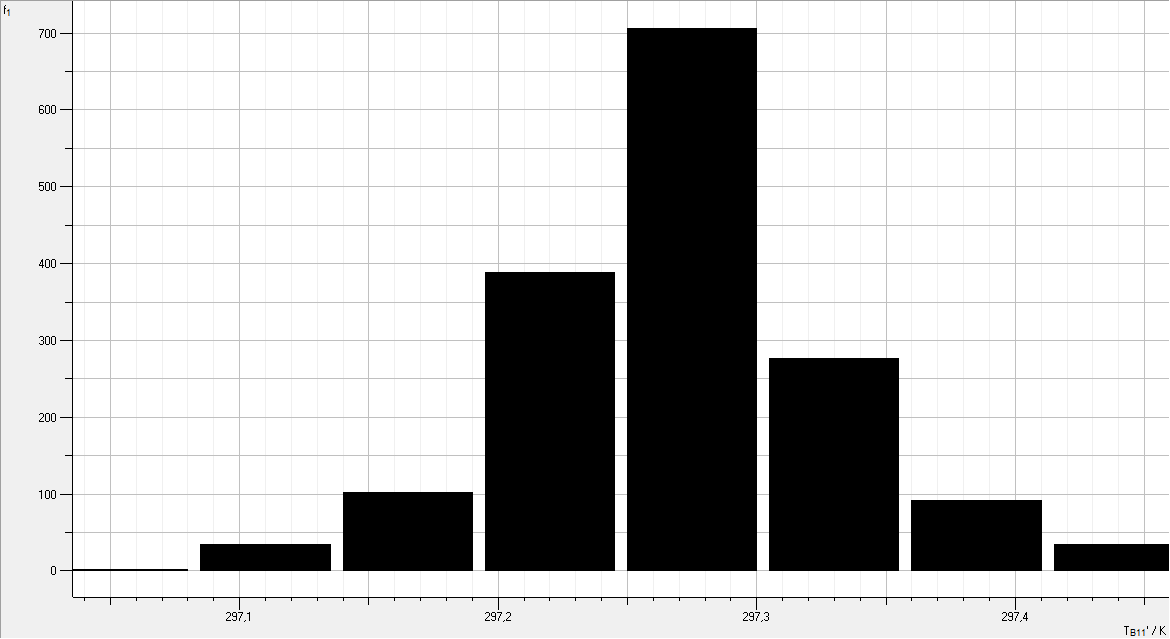
\includegraphics[width=0.49\textwidth]{Bilder/Zimmertemperatur_G1_1.png}}
    \subfigure[Gruppe 2]{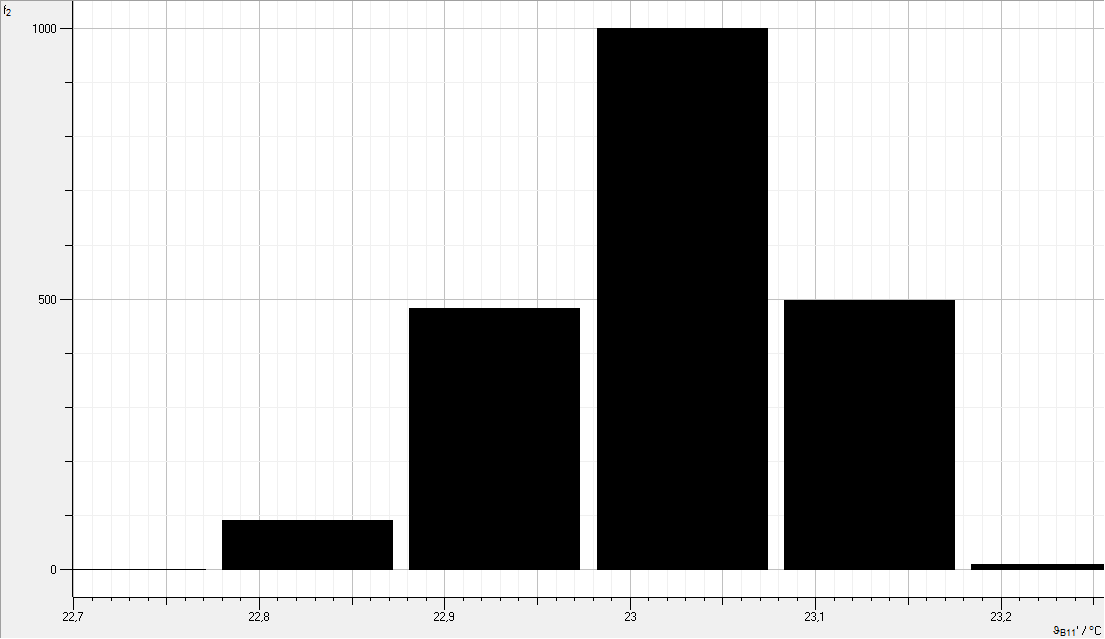
\includegraphics[width=0.49\textwidth]{Bilder/Zimmertemperatur_G2.png}}
\caption{Rauschmessung der Temperatur bei Zimmertemperatur}
\end{figure}

\begin{table}[H]\centering
\caption{Rauschmessung der Temperatur bei Zimmertemperatur}
\begin{tabular}{c|c|c}
 & Gruppe 1 & Gruppe 2 \\ 
\hline 
$T_M$ in K & 297.26 & 296.17 \\ 
$\sigma_T$ in K & 0.054 & 0.069 \\  
\end{tabular} 
\end{table}

Diese Fehler auf die Einzelwerte der Temperatur wurden später als statistische Fehler bei der Hauptmessung verwendet.
\subsection{Rauschmessung der Drucksensoren}
Die Rauschmessung der Drucksensoren wurde jeweils simultan mit der Rauschmessung der Temperatursensoren durchgeführt.


\begin{figure}[H]
    \subfigure[Gruppe 1]{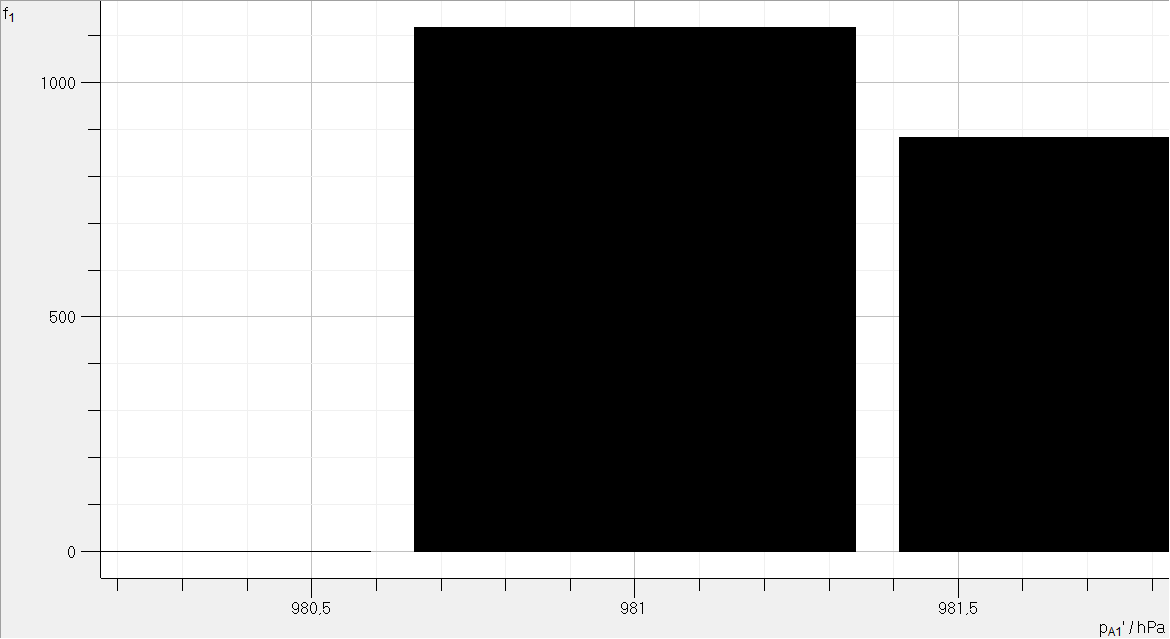
\includegraphics[width=0.49\textwidth]{Bilder/Zimmertemperatur_Druck_G1_1.png}}
    \subfigure[Gruppe 2]{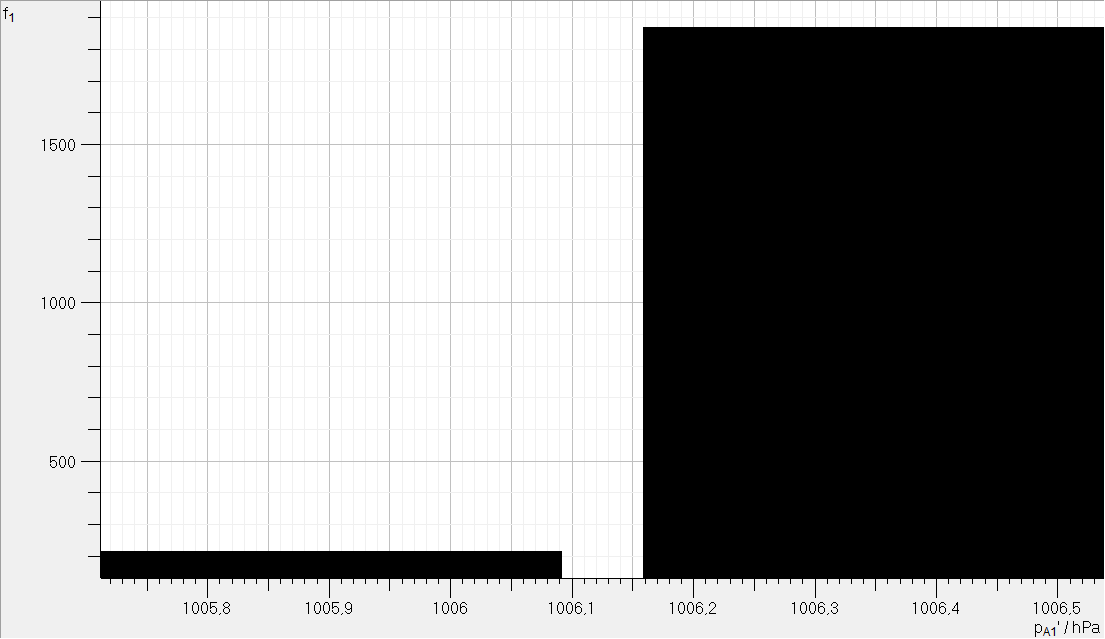
\includegraphics[width=0.49\textwidth]{Bilder/Zimmertemperatur_Druck_G2.png}}
\caption{Rauschmessung des Drucks bei Zimmertemperatur}
\end{figure}

\begin{table}[H]\centering
\caption{Rauschmessung des Drucks bei Zimmertemperatur}
\begin{tabular}{c|c|c}
 & Gruppe 1 & Gruppe 2 \\ 
\hline 
$P_M$ in hPa & 981.443 & 1006.265 \\ 
$\sigma_P$ in hPa & 0.370 & 0.348 \\  
\end{tabular} 
\end{table}

Diese Fehler auf die Einzelwerte des Drucks wurden später als statistische Fehler bei der Hauptmessung und bei der Vermessung der Dichtigkeit verwendet.
\newpage
\section{Kalibrierung des Temperatursensors - Vorversuch}
Da wir bei der Hauptmessung einen Temperatursensor verwenden und nicht genau wissen, ob die angezeigte Temperatur am Cassy auch der tatsächlichen Temperatur entspricht, bestimmen wir in diesem Versuch den systematischen Fehler durch die Kalibrierung des Temperatursensors.

Beide Gruppen haben für die Kalibrierung des Temperatursensors  eine Rauschmessung mit Eiswasser in einem offenen Behälter durchgeführt. \newline
Bevor die tatsächliche Hauptmessung (Abkühlung) gemessen werden konnte, musste das Wasser zunächst auf Siedetemperatur erhitzt werden. Diese Temperatur ist sehr konstant und ist also gut geeignet, um ein Rauschen zu messen und damit die Temperatursensoren zu kalibrieren. \newline
Leider hat Gruppe 1 ihre Rauschmessung bei Siedetemperatur auf Geheiß eines Tutors verworfen \glqq for your eyes only\grqq.
Deshalb mussten wir hier allein auf die Messdaten von Gruppe 2 zurückgreifen.

\begin{figure}[hbtp]
\centering
\includegraphics[scale=0.5]{Bilder/Kalibration_Eiswasser.png}
\caption{Rauschmessung bei Eiswasser}
\end{figure}

\begin{table}[H]\centering
\caption{Rauschmessung der Temperatur beim Gefrierpunkt}
\begin{tabular}{c|c}
$T_M$ in K & 274.277  \\ 
$\sigma_T$ in K & 0.103  \\  
$\sigma_{T_M}$ in K & 0.002 \\  
$T_{Theo}$ & 272.2 \\
\end{tabular} 
\end{table}

\begin{figure}[H]
\centering
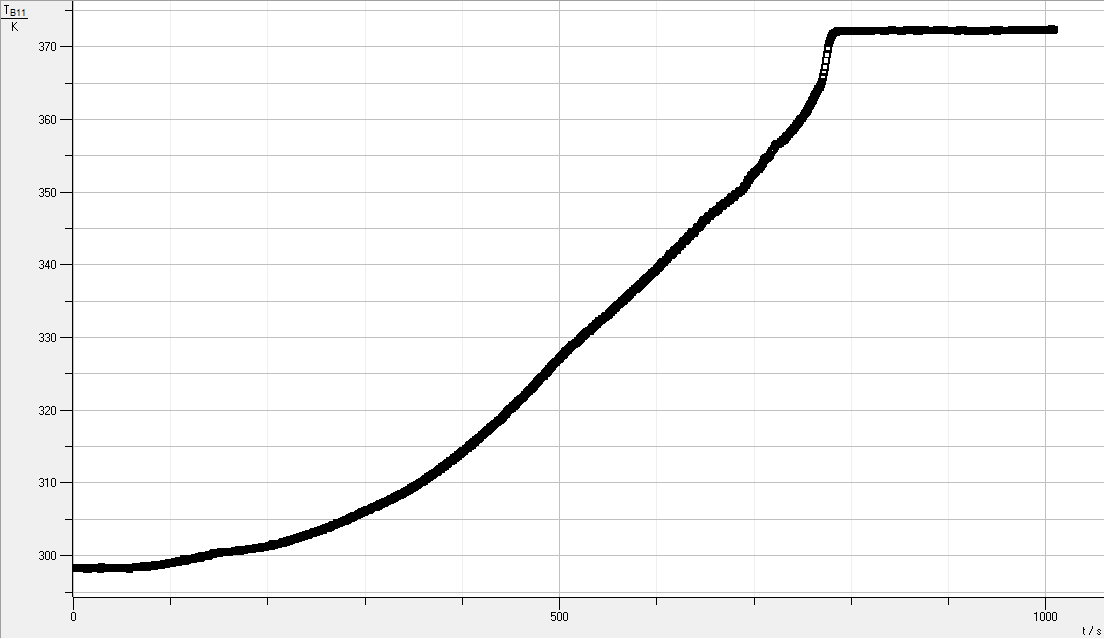
\includegraphics[scale=0.5]{Bilder/heizen.png}
\caption{Heizvorgang. Die Siedetemperatur ist erreicht, wenn die Kurve abflacht.}
\end{figure}

\begin{figure}[H]
\centering
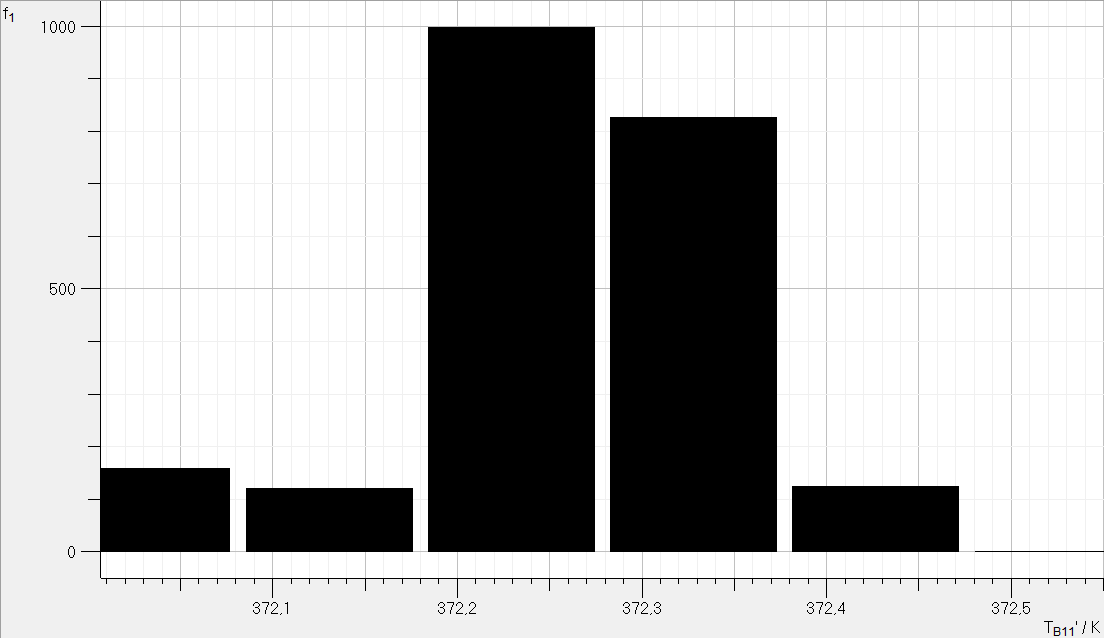
\includegraphics[scale=0.5]{Bilder/heizen_histogramm.png}
\caption{Kalibrierung bei Siedetemperatur.}
\end{figure}


\begin{table}[H]\centering
\caption{Rauschmessung der Temperatur beim Siedepunkt.}
\begin{tabular}{c|c}
$T_M$ in K & 372.227  \\
$\sigma_T$ in K & 0.083  \\
$\sigma_{T_M}$ in K & 0.002 \\
$T_{Theo}$ in K & 372.5 \\
\end{tabular} 
\end{table}
Der theoretische Wert für die Siedetemperatur ergibt sich aus dem Druck. Gemessen hat das Cassy bei Normalbedingungen im Labor einen Wert von: $p_C=1006.5$hPa. Die Wetterstation gab allerdings einen Wert von $p_W=984$hPa an. Also eine Differenz von $22.5$ hPa. Beim Sieden haben wir einen Druck von $1015 hPa$ gemessen. Mit der Korrektur von der Wetterstation ergibt sich also ein Druck von $p_{siede}=992.5hPa$. Bei diesem Druck ist eine Siedetemperatur von $99.4^{\circ}$ C zu erwarten, also 372.5K.  
\begin{figure}[H]
\centering
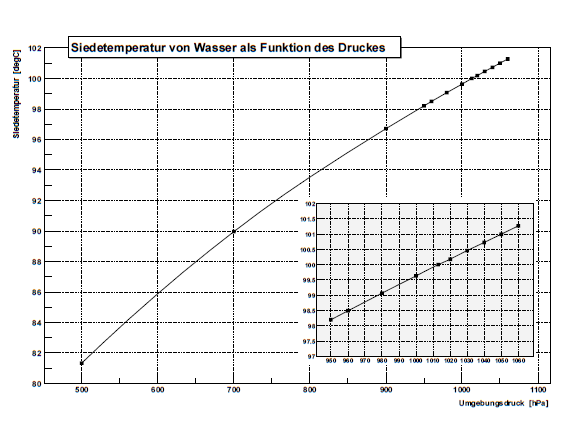
\includegraphics[scale=1]{Bilder/SiedeTemp_Druck.PNG}
\caption{Grafik aus dem Skript. Bei 992.5 hPa ist die Siedetemperatur 99.4 C.}
\end{figure}



Um nun von den von Cassy gemessenen Werte $T_C$ mit Fehlern $\sigma_{T_M}$ auf die realen Werte $T_R$ und ihre Fehler $\sigma_{T_{R}}$ zu kommen trägt man die theoretischen Werte gegen die gemessenen auf. Aus der Steigung und dem y-Achsen-Abschnitt ließe sich dann eine Umrechnung bestimmen.
\begin{equation}
T_{R}=aT_{C}+b
\end{equation}
Hätte man eine solche Formel könnte man durch Fehlerfortpflanzung den Fehler auf den realen  Messwert berechnen. 
\begin{equation}
\sigma_{T_{R}} = \sqrt{(T_C \sigma_a)^2+\sigma_b^2}
\end{equation}
Haben wir diesen Fehler können wir berechnen wie sich dieser dann auf die Werte der Hauptmessung niederschlägt und daraus die systematischen Fehler durch die Temperaturkalibrierung bestimmen. 
\begin{equation}
\sigma_{\lambda_{T}}=\frac{\sigma_T}{T}\cdot \Lambda
\end{equation}
Über eine Lineare Regression durch $T_{Schmelz}$ und $T_{Siede}$ mit ihren Fehlern legt kann man eine solche gesuchte Funktion finden. 
Damit die Werte beim Auftragen von $T_R$ gegen $T_C$ für Steigung und Y-Achsenabschnitt möglichst unkorreliert sind, verschieben wir die Y-Achse um den Mittelwert von Siedetemperatur und Schmelztemperatur.
\begin{equation}
\bar{T}=\frac{T_{Schmelz}+T_{siede}}{2}
\end{equation}
Die theoretischen Werte (y-Werte) sind also nicht fehlerbehaftet, $T_{Schmelz}$ und $T_{Siede}$ (x-Werte) allerdings schon. Leider haben wir in der Praktikumsbibliothek nur eine Funktion gefunden, die entweder Fehler auf beide Achsen akzeptiert oder nur Fehler auf y. \newline 
Deshalb haben wir die Gleichung invertiert und die so gefundene Steigung und Y-Achsenabschnitt in die eigentlich Gesuchten umgeformt.
Die eigentliche Gleichung wäre:
\begin{equation}
T_{R}=a_1(T_{C}-\bar{T})+b_1
\end{equation}
Die von uns zunächst bestimmte Gleichung ist:
\begin{equation}
(T_{C}-\bar{T})=a_2T_R+b_2
\end{equation}
\begin{figure}[H]
\centering
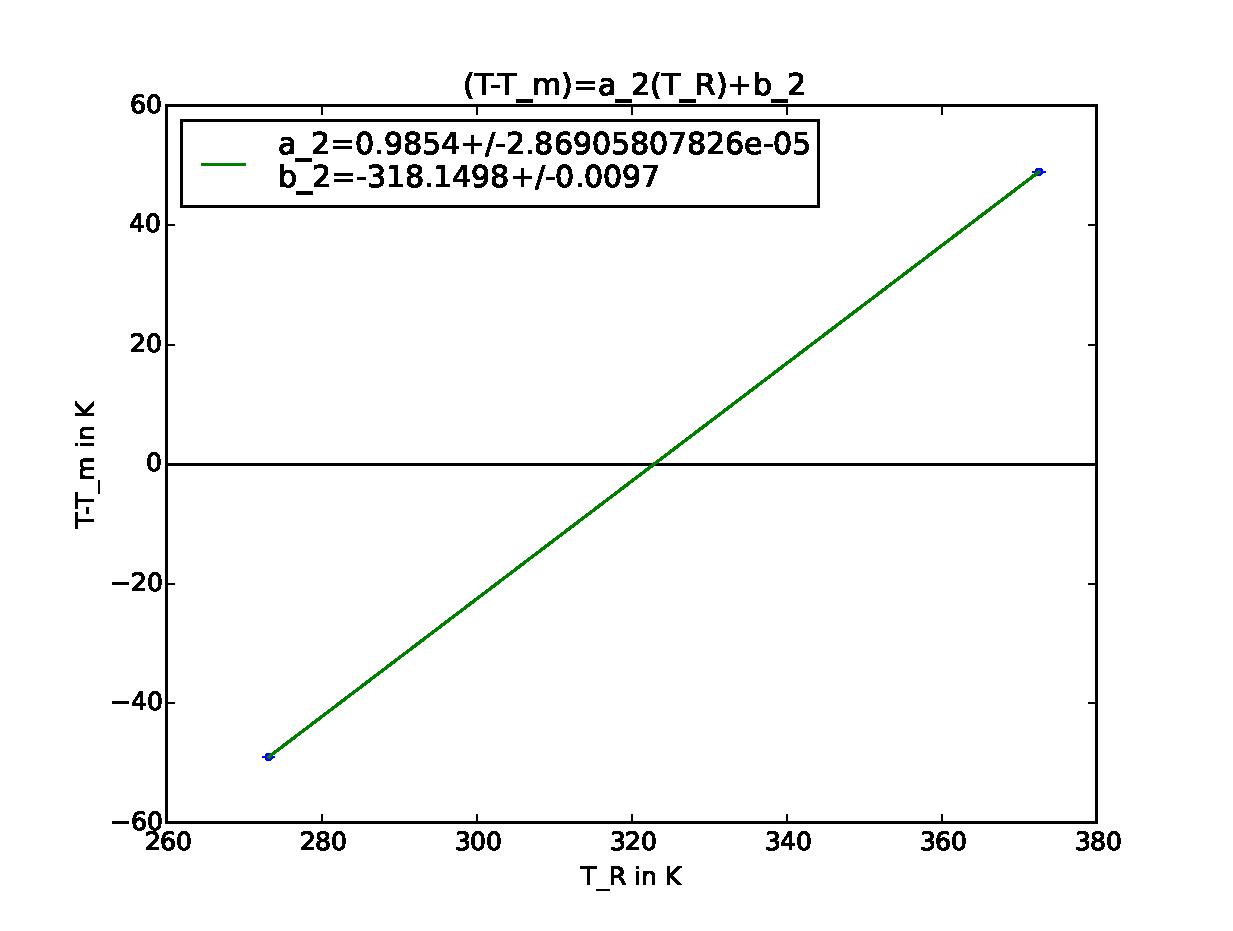
\includegraphics[scale=0.5]{Bilder/lineare_regression_T_kalibration.eps}
\caption{Lineare Regression zur Kalibrierung des Temperatursensors}
\end{figure}

\begin{equation}
a_2=0.985, \hspace{1cm} \sigma_{a_2}=2.870\cdot 10^{-5}\\
\end{equation}
\begin{equation}
b_2=-318.150 K, \hspace{1cm} \sigma_{b_2}=0.010 K
\end{equation}

Da die zweite Gleichung die invertierte der ersten ist, gilt, dass der X-Achsenabschnitt der einen dem Y-Achsenabschnitt der anderen Gleichung entspricht, und dass die eine Steigung die Inverse der anderen Steigung ist.
\begin{equation}
a_1=\frac{1}{a_2}, \hspace{1cm} \sigma_{a_1}=\frac{\sigma_{a_2}}{a_2^2}
\end{equation}
\begin{equation}
b_1=-\frac{b_2}{a_2}, \hspace{1cm} \sigma_{b_1}=b_1 \sqrt{(\frac{\sigma_{b_2}}{b_2})^2+(\frac{\sigma_{a_2}}{a_2})^2}
\end{equation}

Es gilt also:
\begin{equation}
a_1=1.015, \hspace{1cm} \sigma_{a_1}=2.955 \cdot 10^{-5}
\end{equation}
\begin{equation}
b_1=322.86 K, \hspace{1cm} \sigma_{b_1}=0.013 K
\end{equation}

\begin{figure}[H]
\centering
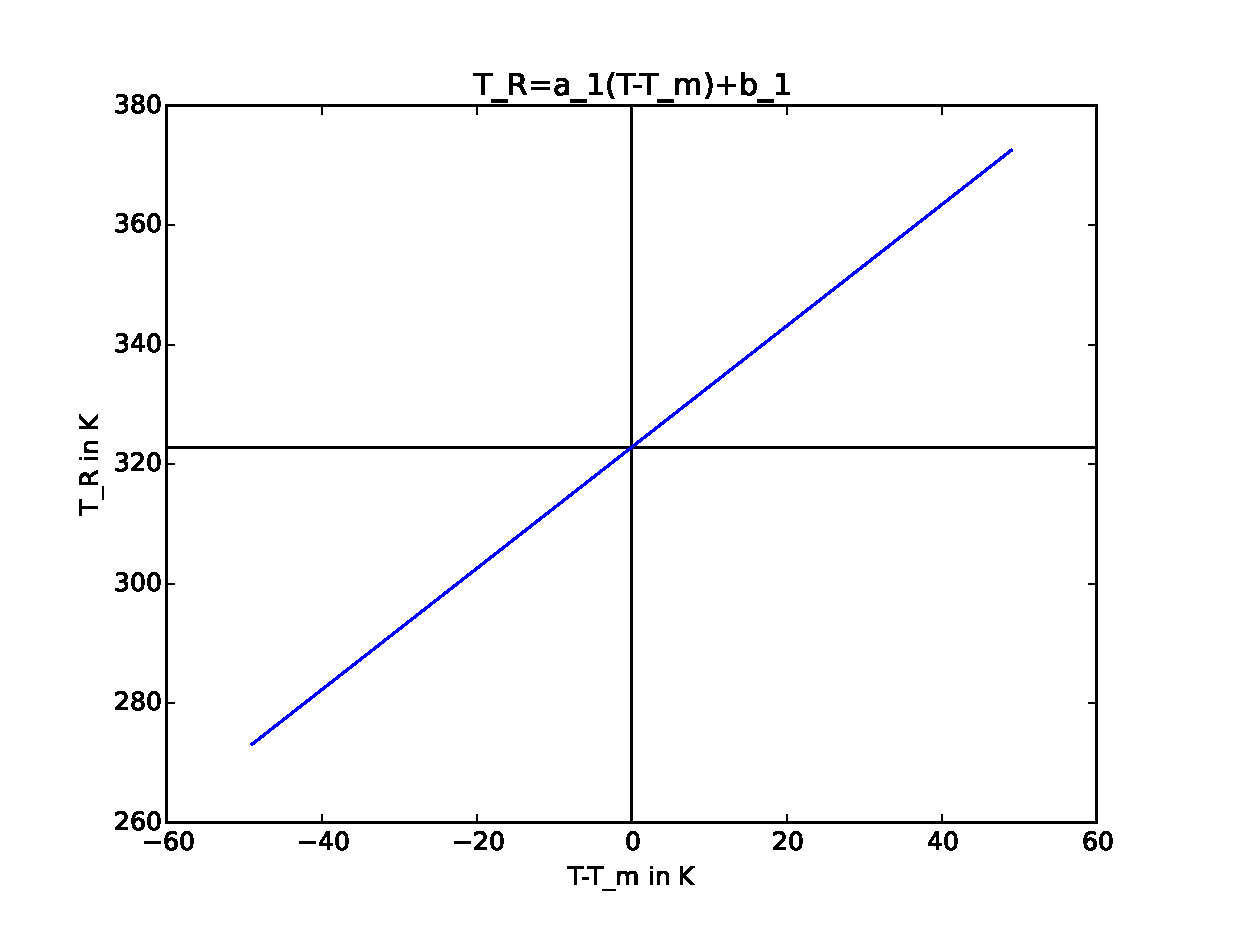
\includegraphics[scale=0.5]{Bilder/gewollteFunktion.eps}
\\
\caption{Funktion zur Kalibrierung}
\end{figure}


Wir haben nun alle Werte um den systematischen Fehler durch die Temperaturkalibrierung und damit den systematischen Fehler auf $\Lambda$ zu bestimmen.

\begin{equation}
\sigma_{T_{R}} = \sqrt{((T_C-\bar{T}) \sigma_a)^2+\sigma_b^2}=0.0137
\end{equation}

\begin{equation}
\sigma_{\lambda_{T}}=\frac{\sigma_T}{T}\cdot \Lambda= \sigma_{Kalibration}
\end{equation}

Aus den Herstellerangaben ergaben sich weitere systematische Fehler.

\begin{table}[H]\centering
\caption{Systematische Fehler aus Herstellerangaben: Druck}
\begin{tabular}{|c|c|}
\hline 
Linearitätsfehler & $\pm 1\%$ \\ 
\hline 
Sensor & $\pm 1\%$ \\ 
\hline 
Verstärkungsfehler & $\pm 1\%$ \\ 
\hline 
\end{tabular} 
\end{table}


\begin{table}[H]\centering
\caption{Systematische Fehler aus Herstellerangaben: Temperatur}
\begin{tabular}{|c|c|}
\hline 
Sensor & $\pm 2.5 K $ \\ 
\hline 
Konverter & $\pm 1\%$ \\ 
\hline 
\end{tabular}
\end{table}

Diese pflanzen sich wie folgt fort.
\begin{equation}
\sigma_{\Lambda,T} = \frac{\sigma_T}{T}\Lambda
\end{equation}
\begin{equation}
\sigma_{\Lambda,p} = RT\frac{\sigma_p}{p}
\end{equation}

\newpage
\begin{multicols}{2}
\begin{table}[H]\centering
\caption{Systematische Fehler Gruppe 1}
\begin{tabular}{c|c|c|c}
 &$\sigma_{Hersteller}$&$\sigma_{Kalibration}$&$\sigma_{Gesamt}$\\
\hline
$\Lambda_0$&0.513&0.002&0.513\\
$\Lambda_1$&0.519&0.002&0.519\\
$\Lambda_2$&0.534&0.002&0.534\\
$\Lambda_3$&0.515&0.002&0.515\\
$\Lambda_4$&0.526&0.002&0.526\\
$\Lambda_5$&0.537&0.002&0.537\\
$\Lambda_6$&0.532&0.002&0.532\\
$\Lambda_7$&0.53&0.002&0.53\\
$\Lambda_8$&0.513&0.002&0.513\\
$\Lambda_9$&0.547&0.002&0.547\\
$\Lambda_{10}$&0.517&0.002&0.517\\
$\Lambda_{11}$&0.514&0.002&0.514\\
$\Lambda_{12}$&0.535&0.002&0.535\\
$\Lambda_{13}$&0.563&0.002&0.563\\
$\Lambda_{14}$&0.499&0.002&0.499\\
$\Lambda_{15}$&0.506&0.002&0.506\\
$\Lambda_{16}$&0.521&0.002&0.521\\
$\Lambda_{17}$&0.488&0.002&0.488\\
$\Lambda_{18}$&0.528&0.002&0.528\\
$\Lambda_{19}$&0.458&0.001&0.458\\
$\Lambda_{20}$&0.468&0.001&0.468\\
\end{tabular}
\end{table}
\begin{table}[H]\centering
\caption{Systematische Fehler Gruppe 2}
\begin{tabular}{c|c|c|c}
 &$\sigma_{Hersteller}$&$\sigma_{Kalibration}$&$\sigma_{Gesamt}$\\
\hline
$\Lambda_0$&0.518&0.002&0.518\\
$\Lambda_1$&0.508&0.002&0.508\\
$\Lambda_2$&0.518&0.002&0.518\\
$\Lambda_3$&0.508&0.002&0.508\\
$\Lambda_4$&0.519&0.002&0.519\\
$\Lambda_5$&0.525&0.002&0.525\\
$\Lambda_6$&0.527&0.002&0.527\\
$\Lambda_7$&0.537&0.002&0.537\\
$\Lambda_8$&0.535&0.002&0.535\\
$\Lambda_9$&0.512&0.002&0.512\\
\end{tabular}
\end{table}
\end{multicols}

\section{Kalibrierung des Drucks - Vorversuch}
Bei Zimmertemperatur haben beide Gruppen ihren Drucksensor kalibriert, indem der bei der Rauschmessung des Drucks gemessene Wert mit dem Wert der Wetterstation verglichen wurde.
\begin{table}[H]\centering
\begin{tabular}{|c|c|c|c|}
\hline 
 & $p_{Cassy}$ & $p_{Wetterstation}$ & $\Delta p$ \\ 
\hline 
Gruppe 1 & 981.54 hPa & 985 hPa & 3.46 hPa \\ 
\hline 
Gruppe 2 & 1006.5 hPa & 984 hPa & 22.5 hPa \\ 
\hline 
\end{tabular} 
\end{table}

Diese Abweichungen fallen bei der Hauptmessung allerdings nicht ins Gewicht, weil sie lediglich den Offset erhöhen würden aber nicht die Steigung verändern.
\newpage
\section{Dichtigkeitsmessung - Vorversuch}
\subsection{Versuchsbeschreibung}
Wir vermessen die Dichtigkeit unserer im Hauptversuch verwendeten Apparatur mit Hilfe des Drucksensors und einer Handpumpe, in dem wir einen für den Hauptversuch typischen Unterdruck erzeugen ($\approx$300 hPa) und die Leckrate messen. Wir tragen die Werte für den Druck gegen die Zeit auf und ermitteln die Leckrate (in $\frac{hPa}{min}$) mittels einer Linearen Regression.

\subsection{Versuchsaufbau und Durchführung}
Wir verwenden den selben Versuchsaufbau wie im Hauptversuch, jedoch fügen wir eine Handpumpe dem T-Ventil hinzu. Die Messwerterfassungseinstellung ändern sich nicht gegenüber den anderen Vorversuchen.
Wir erzeugen mit Hilfe der Handpumpe einen Unterdruck und messen den Druck über 10 Minuten. Dieser nimmt linear über die Zeit hinweg zu. Wir messen den Druck und tragen diesen gegen die Zeit auf.
\subsection{Versuchsauswertung}

\subsubsection{Rohdaten}

\begin{figure}[H]
\centering
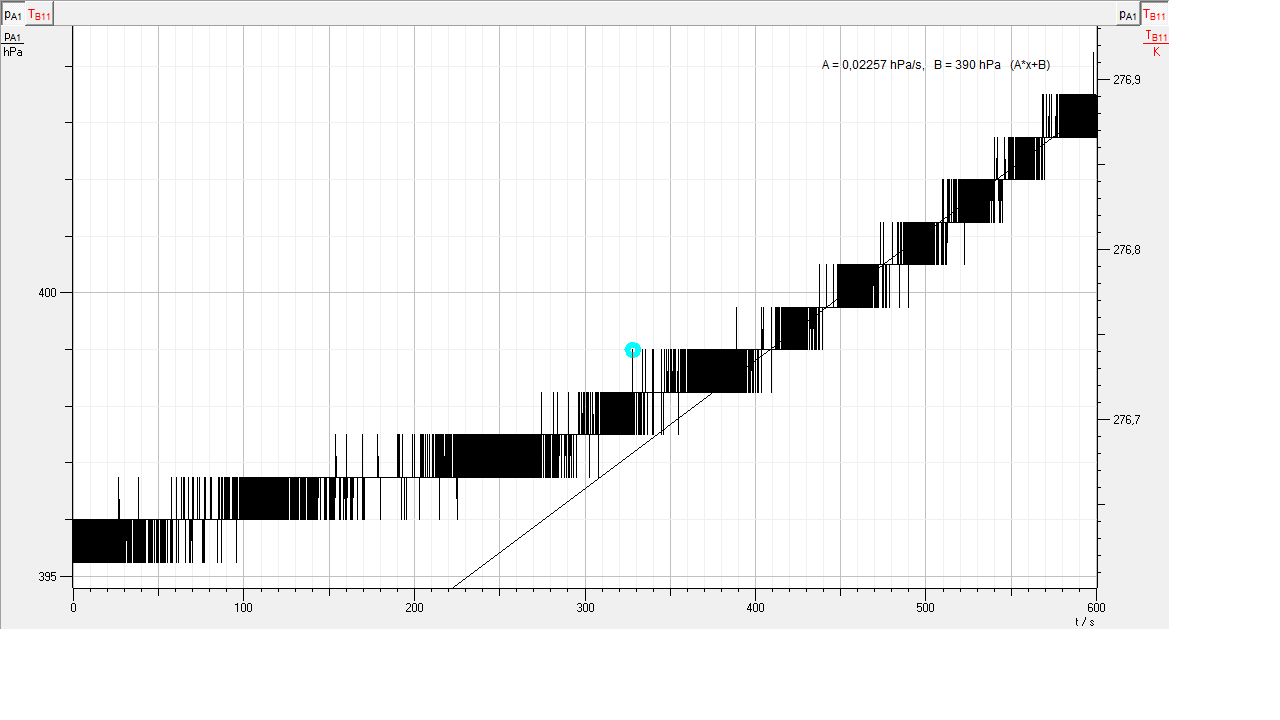
\includegraphics[scale=0.3]{Bilder/dichtigkeit_raw_JM.png}
\caption{Leckmessung Gruppe 1}
\end{figure}

\begin{figure}[H]
\centering
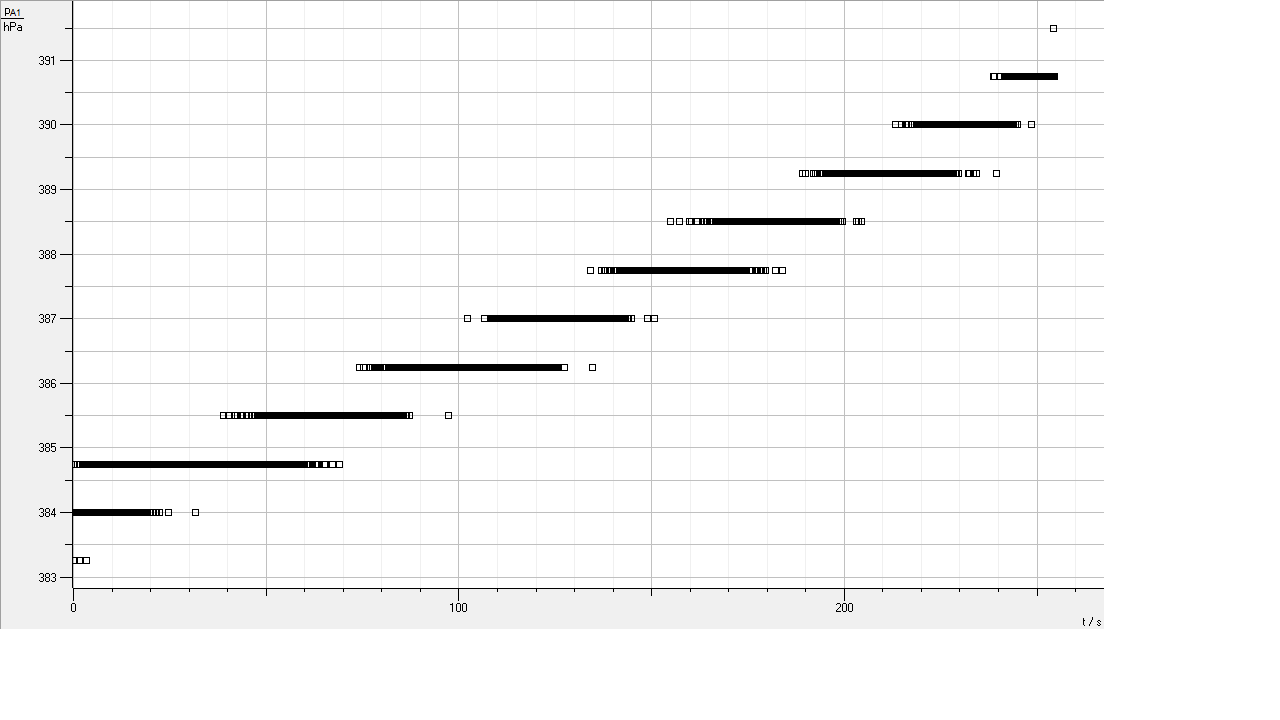
\includegraphics[scale=0.3]{Bilder/dichtigkeit_raw_EL.png}
\caption{Leckmessung Gruppe 2}
\end{figure}

\subsubsection{Transformation und Analyse der Rohdaten}

Bei Gruppe 1 haben wir am Anfang eine sich ändernde Leckrate festgestellt, die zunächst bei $\approx$0.7$\,\frac{hPa}{min}$ lag. Diese pendelte sich gegen Ende der Messung bei 1.264$\,\frac{hPa}{min}$ ein. Daher haben wir vor der Linearen Regression die Werte vom Anfang abgeschnitten. Wir führen eine Lineare Regression durch und erhalten aus der Steigung die Leckrate.

\begin{figure}[H]
\centering
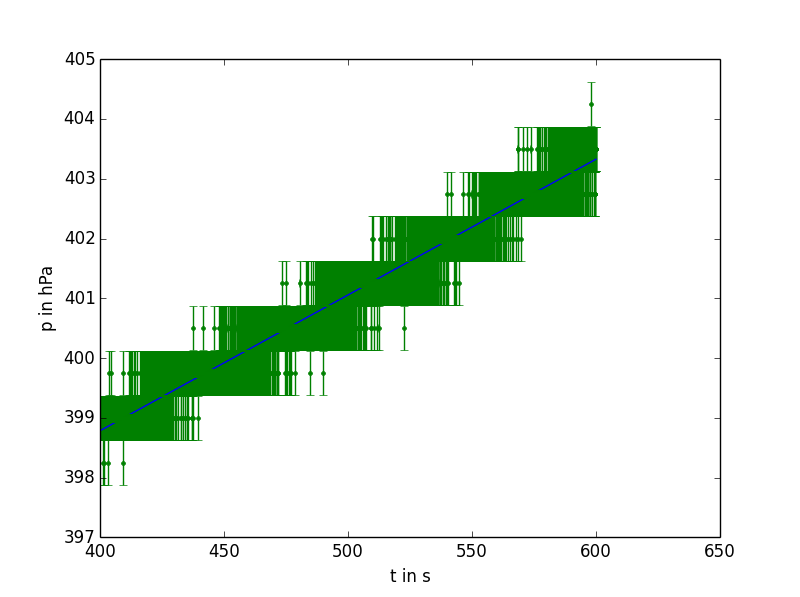
\includegraphics[scale=0.5]{Bilder/dichtigkeit__JM.png}
\caption{Lineare Regression Gruppe 1 $\frac{\chi^2}{f}=0.638$}
\end{figure}

\begin{figure}[H]
\centering
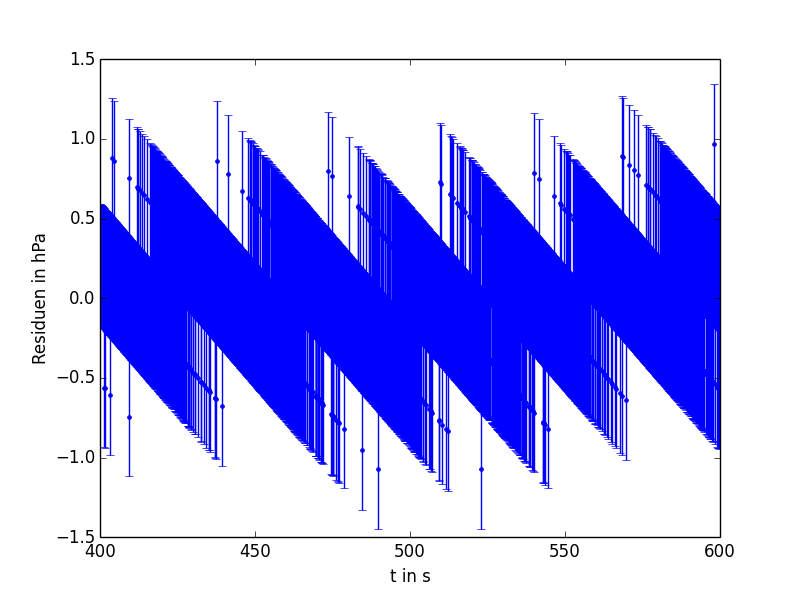
\includegraphics[scale=0.5]{Bilder/residuen_dichtigkeit_JM.png}
\caption{Residuen für die Anpassung von Gruppe 1}
\end{figure}

Die Leckrate für Gruppe 1 beträgt 1.364$\,\frac{hPa}{min}$.
\newpage

\begin{figure}[H]
\centering
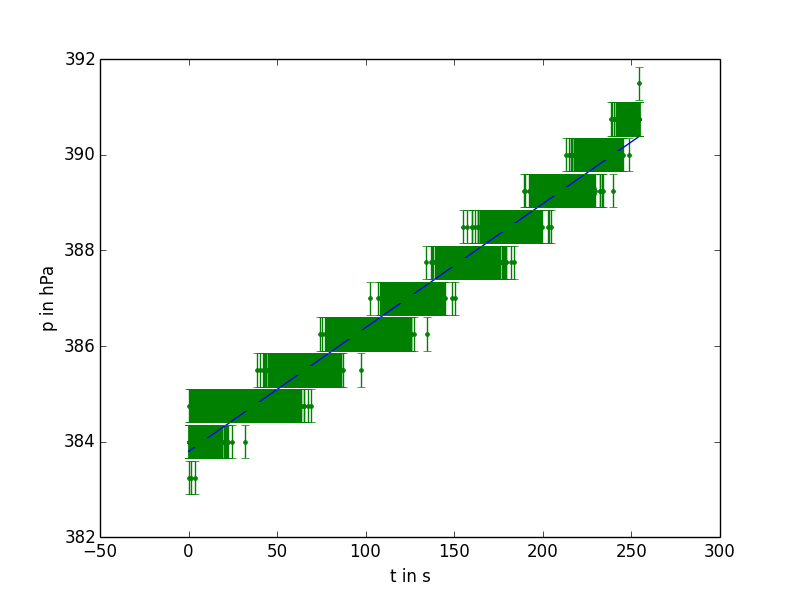
\includegraphics[scale=0.5]{Bilder/dichtigkeit__EL.png}
\caption{Lineare Regression Gruppe 2, $\frac{\chi^2}{f}=0.804$}
\end{figure}

\begin{figure}[H]
\centering
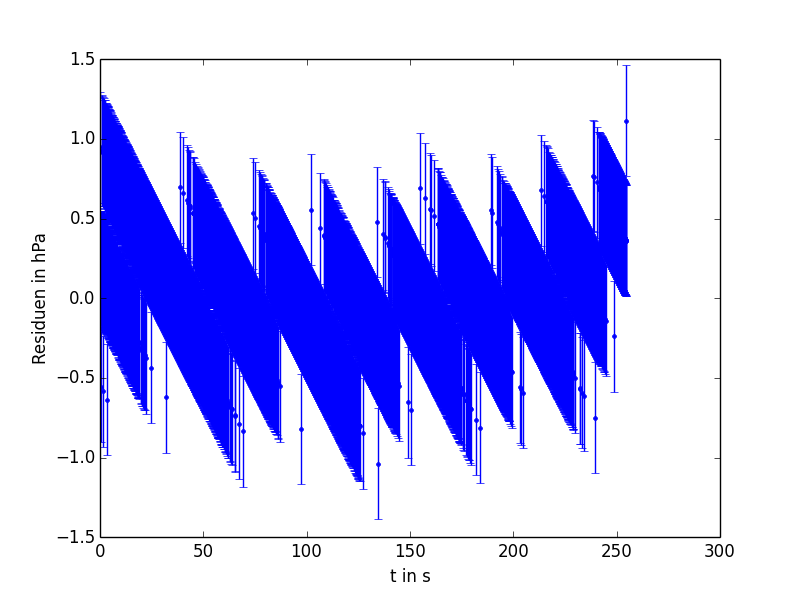
\includegraphics[scale=0.5]{Bilder/residuen_dichtigkeit_EL.png}
\caption{Residuen der Anpassung Gruppe 2}
\end{figure}

Die Leckrate für Gruppe 2 beträgt 1.554$\,\frac{hPa}{min}$.

\subsubsection{Fazit}
Die Leckraten von 1.364$\,\frac{hPa}{min}$, bzw 1.554$\,\frac{hPa}{min}$ betragen nur ca $\frac{1}{300}$ unseres eigentlichen Wertes. Da die Lineare Regression in einem Bereich stattgefunden hat, in dem wir mir der Aulösung des Sensors arbeiten mussten, sieht man diese Bereich sehr gut in den Residuenplots. Ansonsten lassen sich keine Systematiken feststellen. Wir sind mit den Ergebnissen des Vorversuchs zufrieden, die Güte der Anpassung liegt ebenfalls in einem zufriedenstellenden Rahmen ($\frac{\chi^2}{f}=0.638$ für Gruppe 1 und $\frac{\chi^2}{f}=0.804$ für Gruppe 2).
\newpage
\section{Bestimmung der Verdampfungsenthalpie von Wasser}
\subsection{Versuchsaufbau und Durchführung}
%Genaue Beschreibung der verwendeten Aufbauten unter Verwendung von %Skizzen oder Photos
%Beschreibung der Messwerterfassungseinstellungen (eingestellte %Messzeiten, Messbedingungen,
%5Trigger, Anzahl der Messungen) und der Durchführung der Versuche. (max. 1 Seite)
\begin{figure}[H]
\centering
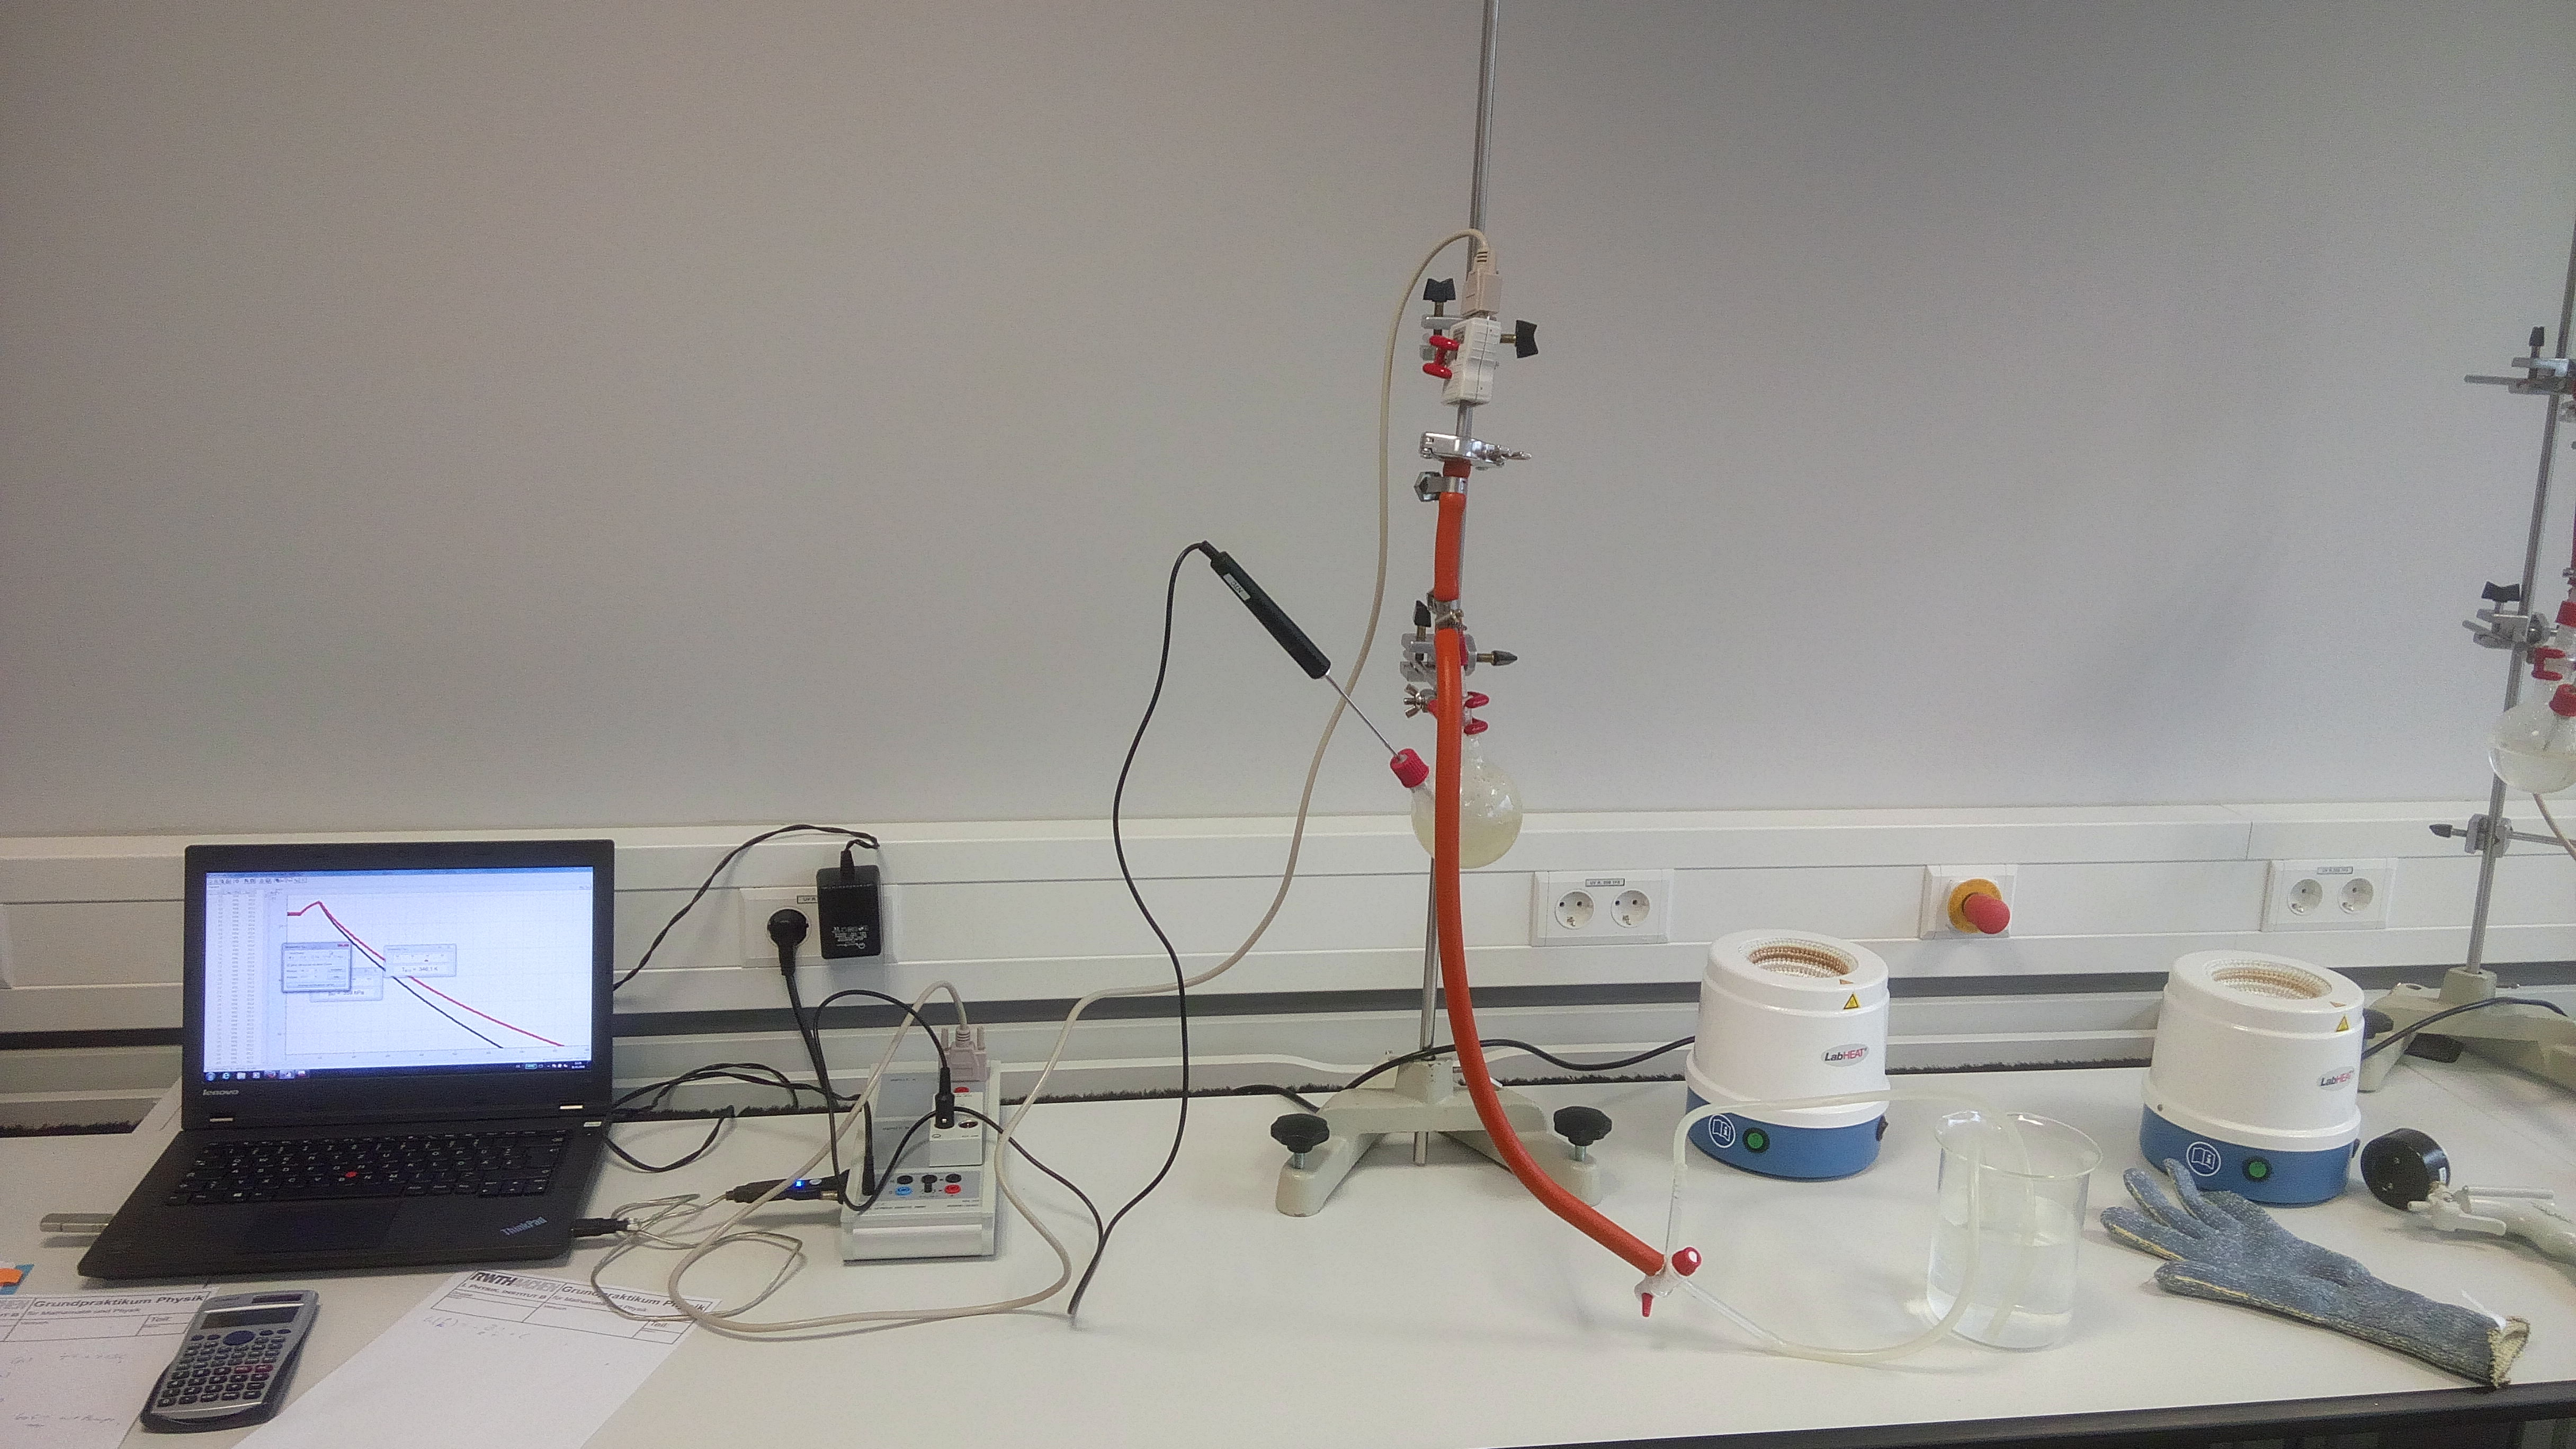
\includegraphics[scale=0.1]{Bilder/IMG_20160331_121650.jpg}
\caption{Versuchsaufbau während des Abkühlvorgangs}
\end{figure}
Benötigte Geräte:
\begin{multicols}{2}
\begin{itemize}
\item Sensor-Cassy
\item Heizhaube
\item Absolutdrucksensor mit Stativstange
\item Verbindungskabel
\item Temperatursensor
\item Temperaturbox
\columnbreak
\item Kolben
\item Messbecher
\item Glasventil
\item Stativ mit Stange
\item Schläuche
\item Verbindungsstücke
\item Muffen
\end{itemize}
\end{multicols}
\begin{table}[H]\centering \caption{Messparameter} \begin{tabular}{ccc} & Gruppe 1 & Gruppe 2 \\ \hline Intervall & 50ms & 100ms \\ Anzahl & 12000 & unbegrenzt \\ Messzeit & 600s & unbegrenzt \\ \end{tabular} \end{table}
Für diesen Versuch wurde der bereits mit Wasser befüllte Kolben nun mit Hilfe der Heizhaube erhitzt. Während des Erhitzens wurde das Ventil so gestellt, dass der Druck durch einen Schlauch in den Messbecher geleitet wurde, der vorher ebenfalls mit Wasser befüllt wurde. Dadurch wurde verhindert dass Luft zurück in den Kolben strömen konnte.
Nachdem die Siedetemperatur erreicht und möglichst viel Luft aus dem Kolben durch Wasserdampf verdrängt wurde, haben wir die Heizhaube entfernt, das Ventil geschlossen und die Messung gestartet.
\subsection{Versuchsauswertung}
\subsubsection{Rohdaten}
\begin{figure}[H]
\centering
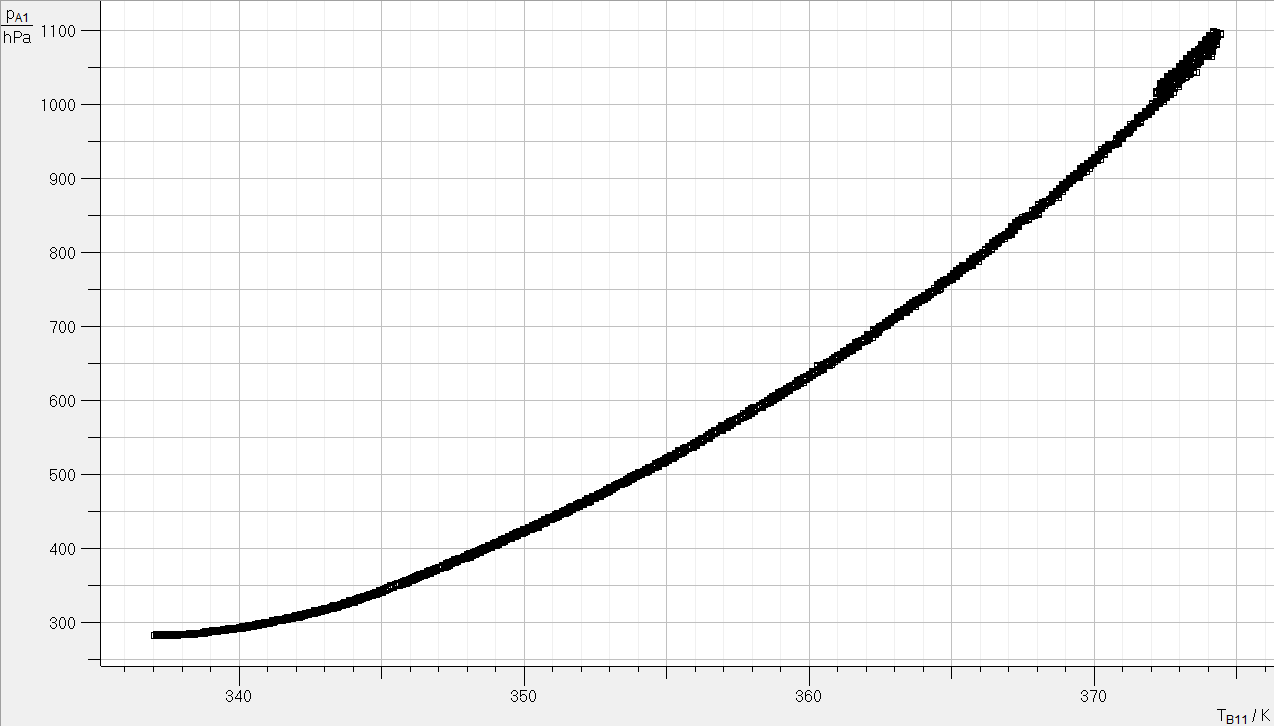
\includegraphics[scale=0.5]{Bilder/RohdatenHaupmessungGrp2.png}
\caption{Druck gegen Temperatur des Abkühlvorgangs Gruppe 2}
\end{figure}
\begin{figure}[H]
\centering
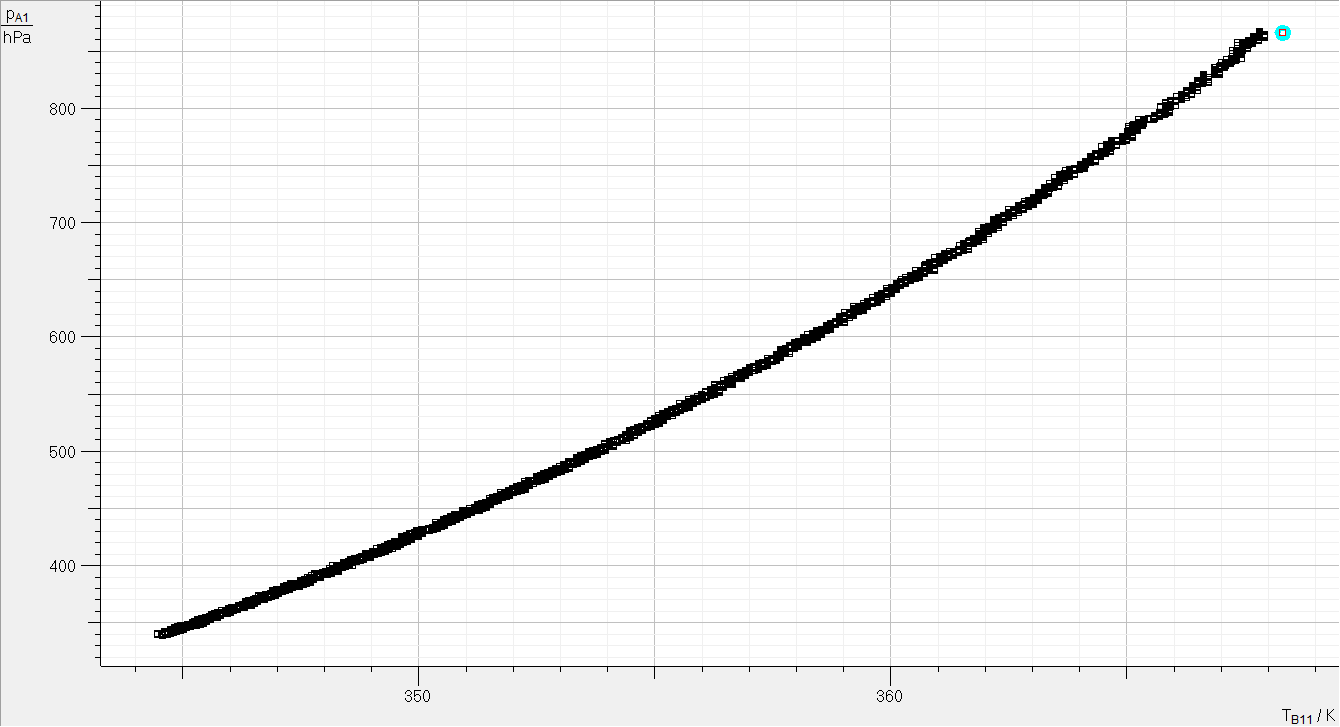
\includegraphics[scale=0.5]{Bilder/RohdatenHaupmessungGrp11.png}
\caption{Druck gegen Temperatur des Abkühlvorgangs Gruppe 1}
\end{figure}
\subsubsection{Transformation der Rohdaten/Analyse}
Zunächst wurden alle Werte unserer Messung umgeformt in $\ln(p)$ und $\frac{1}{T}$.
\begin{figure}[H]
\centering
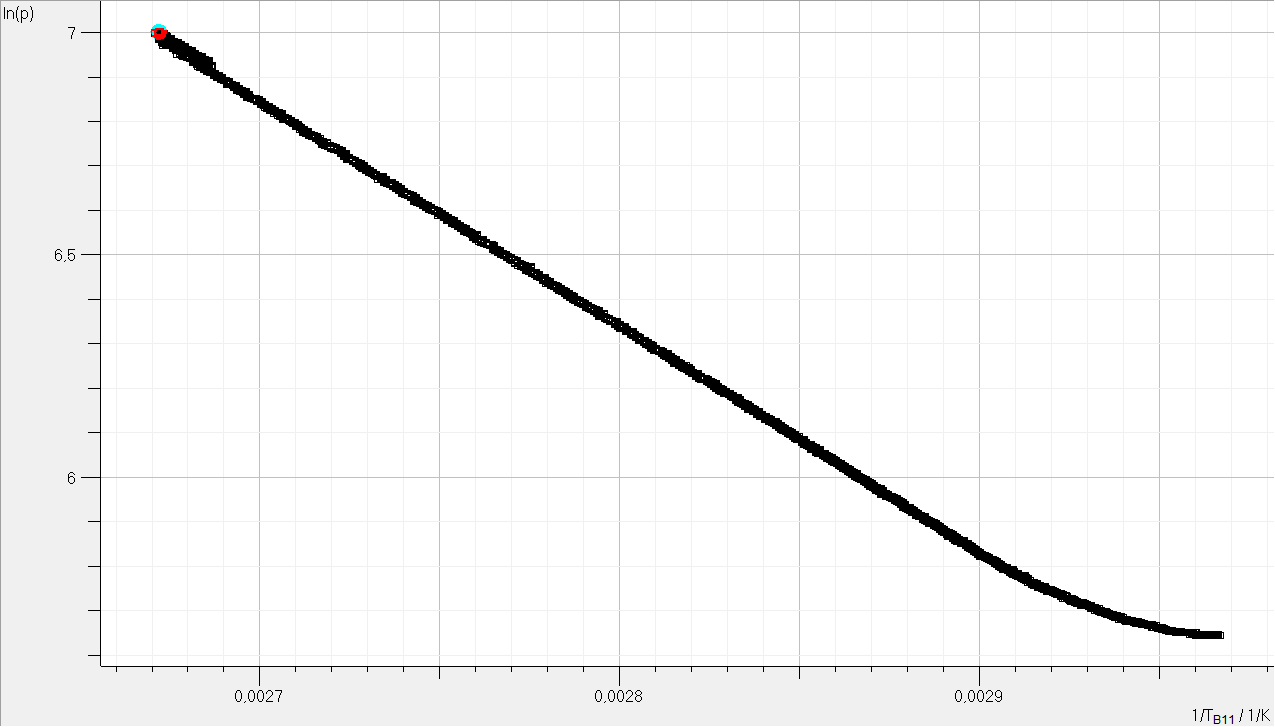
\includegraphics[scale=0.5]{Bilder/HauptmessungbearbeitetGrp2.png}
\caption{$\ln(p)$ gegen $\frac{1}{T}$ des Abkühlvorgangs Gruppe 2}
\end{figure}
Mit diesen Werten wurde anschließend eine Lineare Regression durchgeführt und durch die Werte mit ihren Fehlern geplottet. Dabei wurden die Werte in 16 Teile unterteilt um später die Temperaturabhängigkeit der Verdampfungswärme betrachten zu können.
\begin{figure}[H]
\centering
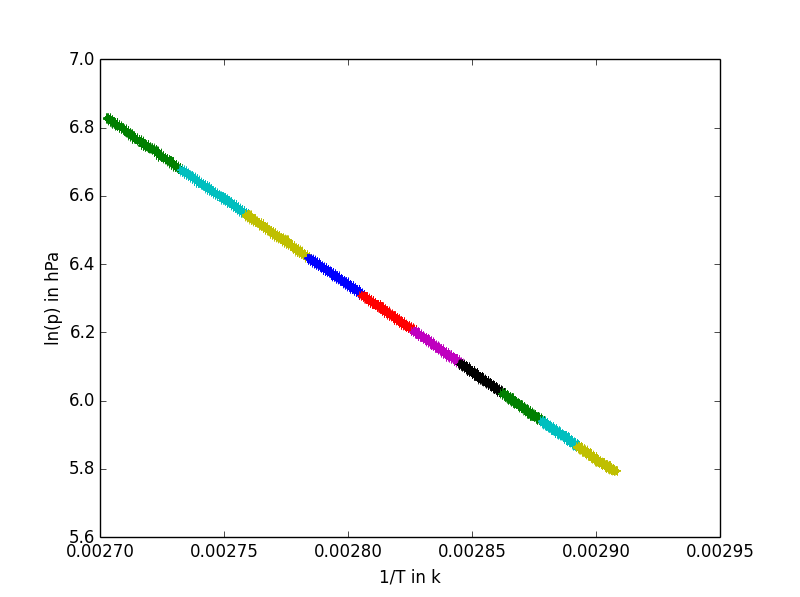
\includegraphics[scale=0.7]{Bilder/linreg_EL_neuerFehler.png}
\caption{Lineare Regression durch die umgeformten Messwerte, Randwerte wurden bereits entfernt Gruppe 2}
\end{figure}
\begin{figure}[H]
\centering
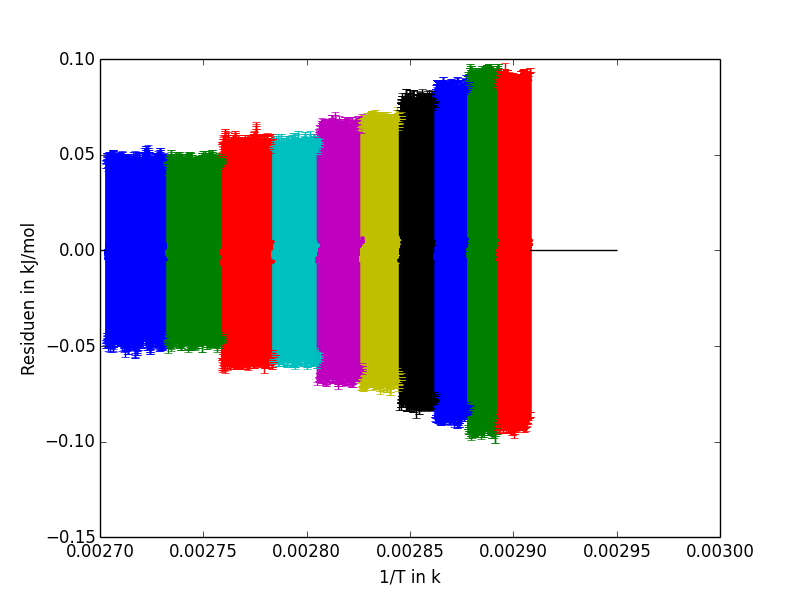
\includegraphics[scale=0.7]{Bilder/residuen_EL_neuerFehler.png}
\caption{Residuen zur Linearen Regression}
\end{figure}
\begin{figure}[H]
\centering
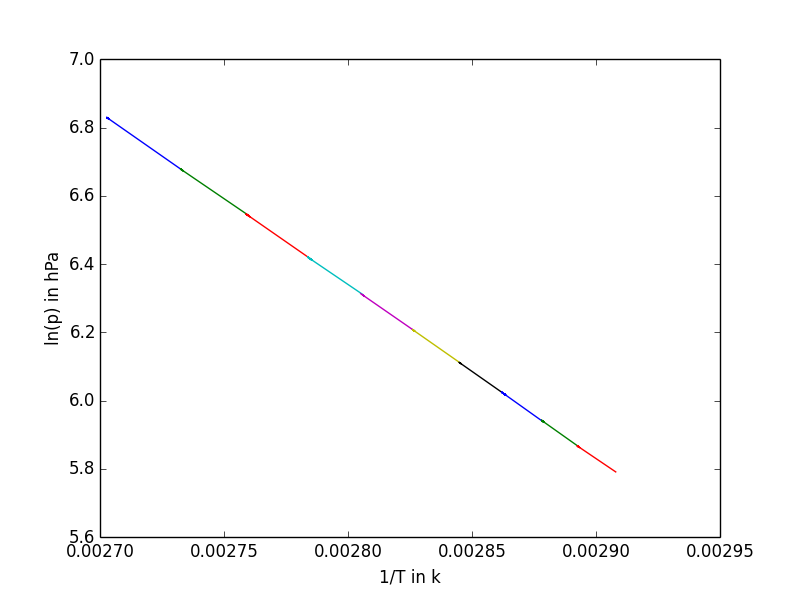
\includegraphics[scale=0.7]{Bilder/linreg_nurlinreg_EL.png}
\caption{Lineare Regression ohne Messwerte Gruppe 2}
\end{figure}
\begin{itemize}
\item $\frac{\chi^2}{f} \Rightarrow 1.27 | 0.96 | 1.12 | 0.86 | 0.89 | 0.77 | 0.79 | 0.78 | 0.71 | 0.74$
\end{itemize}
Die Steigung der Linearen Regression ergibt sich zu $-\frac{\Lambda}{R}$, sodass sich daraus nun unser Ergebnis für $\Lambda$ berechnen lässt.
\begin{table}[H]\centering
\caption{Ergebnisse Gruppe 1}

\begin{tabular}{c|c|c|c|c}
Abschnitt&T in K&$\Lambda$ in $\frac{kJ}{mol}$&$\sigma_{\Lambda_{stat}}$in $\frac{kJ}{mol}$&$\sigma_{\Lambda_{sys}}$in $\frac{kJ}{mol}$\\
\hline
1&366.37&41.74&0.342&0.513\\
2&363.81&42.08&0.327&0.519\\
3&361.65&43.27&0.339&0.534\\
4&359.72&41.62&0.324&0.515\\
5&358.0&42.51&0.327&0.526\\
6&356.39&43.34&0.294&0.537\\
7&354.95&42.88&0.272&0.532\\
8&353.53&42.65&0.365&0.53\\
9&352.27&41.19&0.327&0.513\\
10&351.06&44.01&0.384&0.547\\
11&349.95&41.45&0.395&0.517\\
12&348.87&41.2&0.299&0.514\\
13&347.84&42.88&0.406&0.535\\
14&346.86&45.11&0.432&0.563\\
15&345.91&39.82&0.446&0.499\\
16&344.99&40.41&0.414&0.506\\
17&343.32&41.56&0.143&0.521\\
18&342.4&38.78&0.163&0.488\\
19&341.57&42.03&0.212&0.528\\
20&340.68&36.24&0.175&0.458\\
21&339.78&37.06&0.189&0.468\\
\end{tabular}
\end{table}

\begin{table}[H]\centering
\caption{Ergebnisse Gruppe 2}
\begin{tabular}{c|c|c|c|c}
Abschnitt&T in K&$\Lambda$ in $\frac{kJ}{mol}$&$\sigma_{\Lambda_{stat}}$in $\frac{kJ}{mol}$&$\sigma_{\Lambda_{sys}}$in $\frac{kJ}{mol}$\\
\hline
1&367.93&42.18&0.273&0.518\\
2&364.13&41.17&0.156&0.508\\
3&360.76&41.96&0.102&0.518\\
4&357.71&40.97&0.1&0.508\\
5&355.03&41.8&0.12&0.519\\
6&352.6&42.24&0.117&0.525\\
7&350.38&42.31&0.136&0.527\\
8&348.4&43.03&0.141&0.537\\
9&346.54&42.79&0.162&0.535\\
10&344.83&40.84&0.175&0.512\\
\end{tabular}
\end{table}
Anschließend wurden die Ergebnisse für $\Lambda$ gegen die Temperatur aufgetragen.
\begin{figure}[H]
\centering
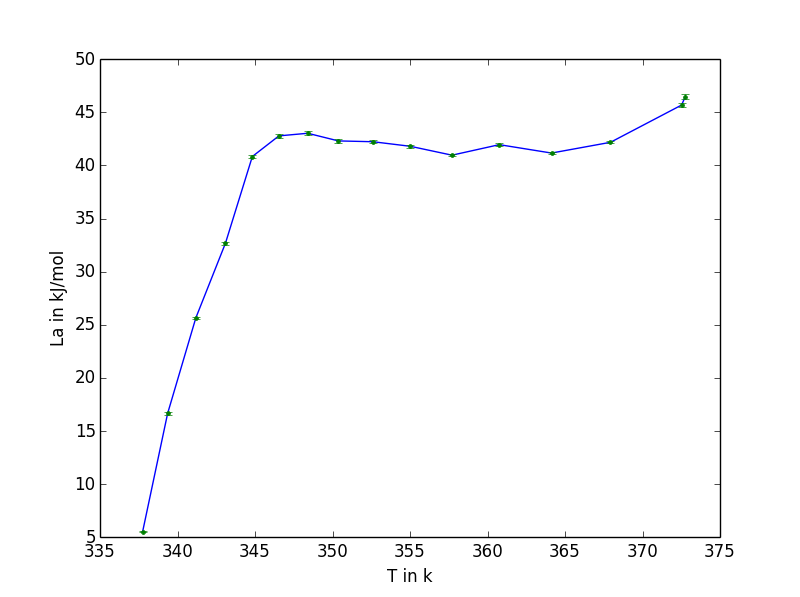
\includegraphics[scale=0.7]{Bilder/lamda_EL_neuerFehler.png}
\caption{Verdampfungswärme gegen Temperatur Gruppe 2}
\end{figure}
Die ersten vier so wie die letzten zwei Werte wurden in allen anderen Plots ausgelassen. Hier sieht man, dass dies sinnvoll war, da diese noch während des Aufheizens bzw. nachdem das Wasser nicht mehr siedete aufgezeichnet wurden. 
\subsubsection{Fazit}
Allgemein lässt sich sagen, dass der Versuch in beiden Gruppen sehr gut abgelaufen ist. Das Abdichten hat gut geklappt und das Aufheizen sowie das Vermessen der Daten beim Abkühlen hat keine Probleme gemacht.
Die Anpassung unserer Linearen Regressionen durch die Messwerte waren nach den $\frac{\chi^2}{f}$ zu urteilen, sinnvoll.
Die errechneten Werte für $\Lambda$ liegen alle in der gleichen Größenordnung wie der im Skript angegebene Literaturwert von $40.6 \frac{kJ}{mol}$.
Wenn man die Werte mit der Tabelle(\ref{lambdaskirpt}) vergleicht, liegen die Abweichungen zwischen 1 und 10 $\sigma$. 
Die Auftragung von $\Lambda$ gegen $T$ liefert leider kein sinnvolles Ergebnis, was wohl an den Näherungen in den benutzten Gleichungen liegt.
Beispiele dafür sind: Ideale Gasgleichung, Vernachlässigen des Wasservolumens und das Vernachlässigen der Volumenänderung beim Erhitzen bzw. Abkühlen.

\section{Anhang}
\begin{figure}[H]
\centering
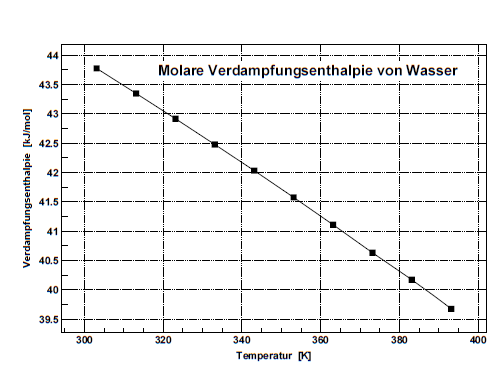
\includegraphics[scale=0.7]{Bilder/Verdampfungsentalpie.PNG}
\label{lambdaskirpt}
\caption{Verdampfungsentalpie gegen Temperatur aus dem Skript}
\end{figure}
\begin{figure}[H]
\centering
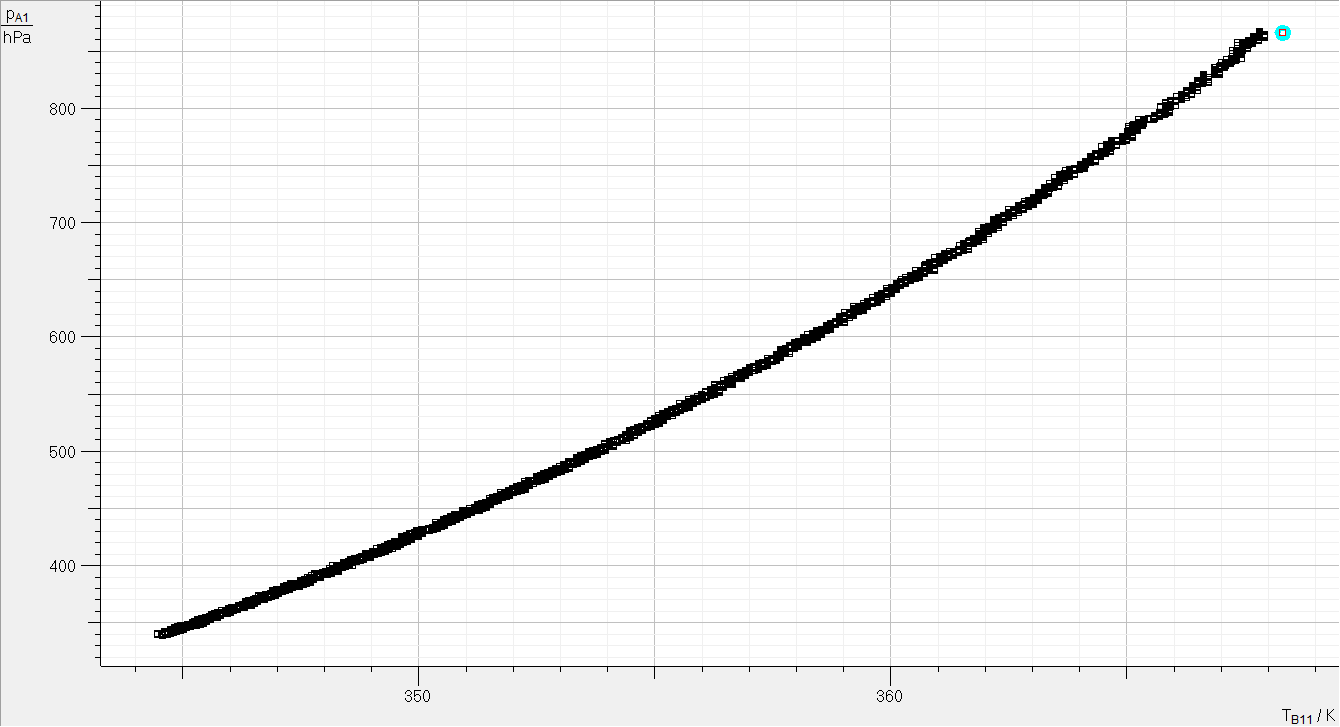
\includegraphics[scale=0.5]{Bilder/RohdatenHaupmessungGrp11.png}
\caption{1. Rohdaten Gruppe 1}
\end{figure}
\begin{figure}[H]
\centering
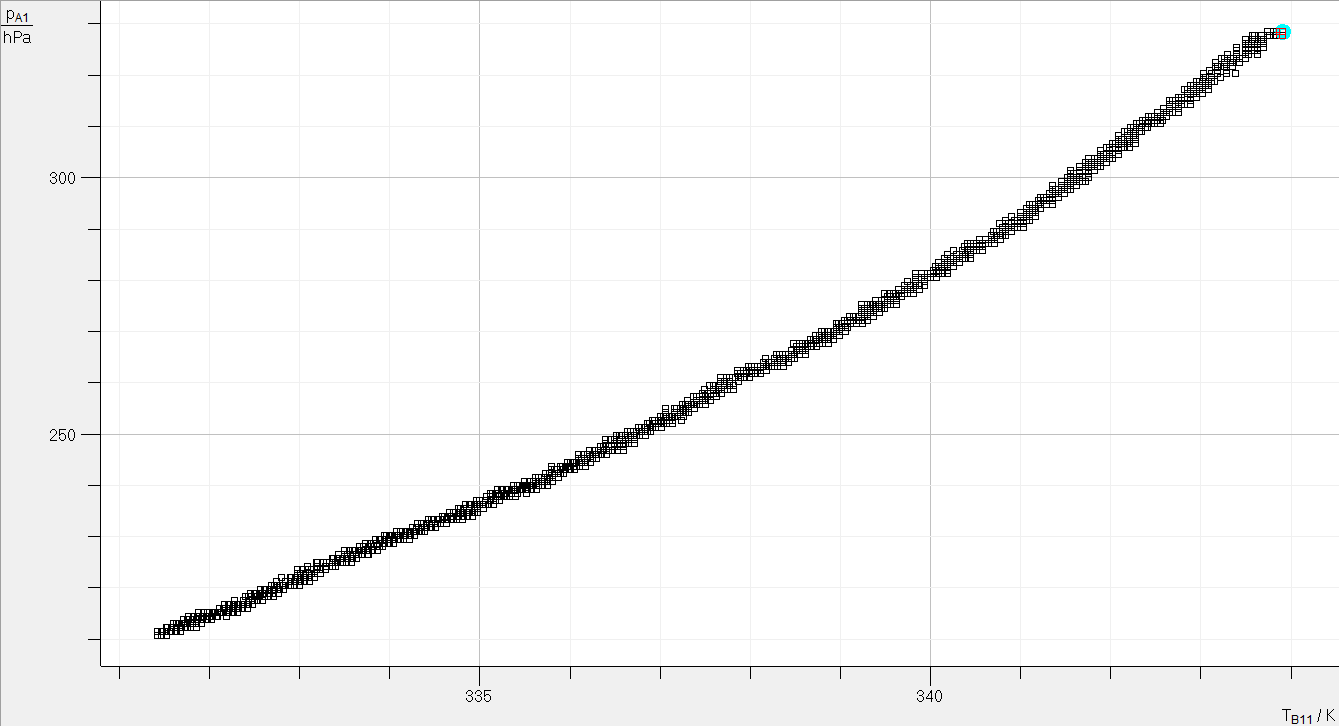
\includegraphics[scale=0.5]{Bilder/RohdatenHaupmessungGrp12.png}
\caption{2. Rohdaten Gruppe 1}
\end{figure}
\begin{figure}[H]
\centering
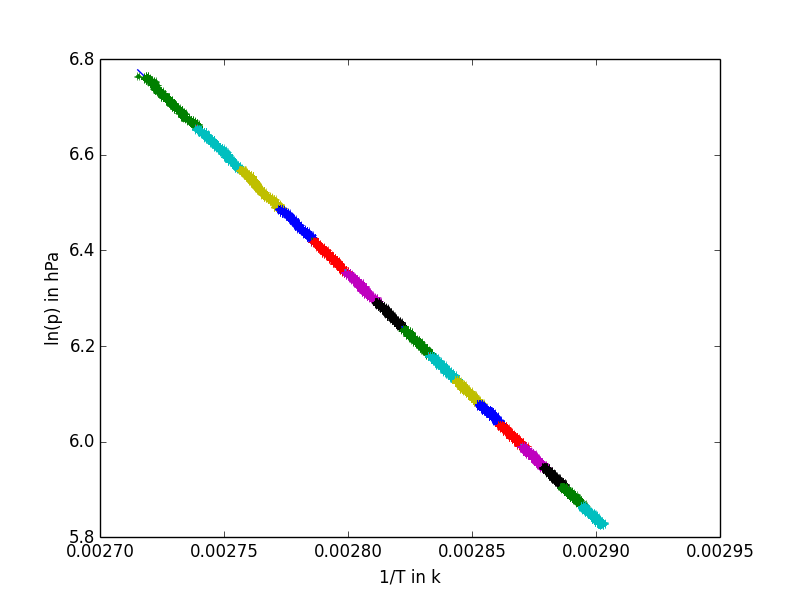
\includegraphics[scale=0.7]{Bilder/linreg_lambda_JM_1.png}
\caption{1. Lineare Regression Hauptmessung Gruppe 1}
\end{figure}
\begin{figure}[H]
\centering
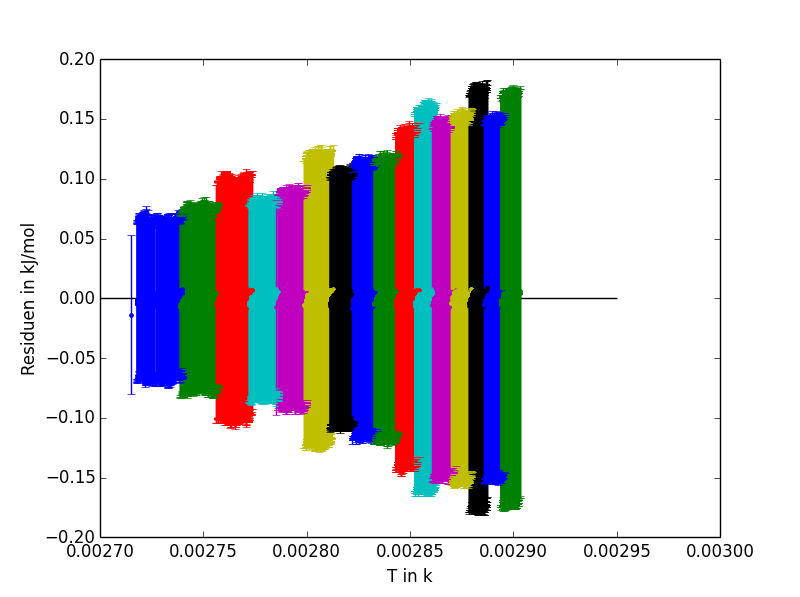
\includegraphics[scale=0.7]{Bilder/residuen_JM_1.png}
\caption{Residuen zur 1. Linearen Regression Hauptmessung Gruppe 1}
\end{figure}
\begin{figure}[H]
\centering
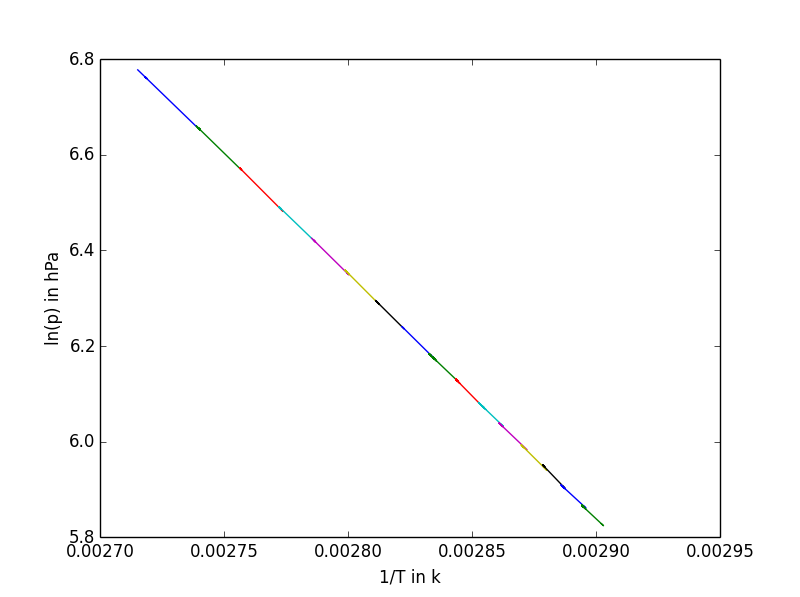
\includegraphics[scale=0.7]{Bilder/linreg_nurlinreg_JM_1.png}
\caption{1. Lineare Regression Hauptmessung Gruppe 1 ohne Messwerte}
\end{figure}
\begin{figure}[H]
\centering
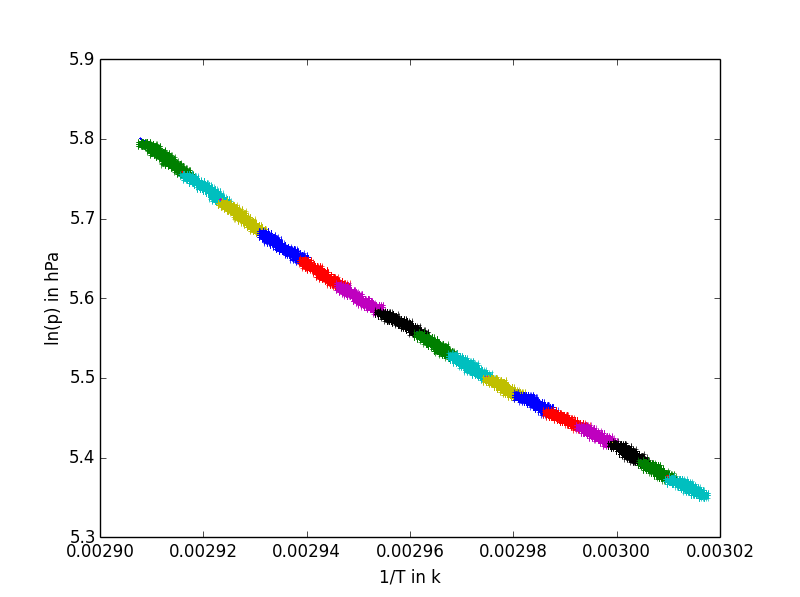
\includegraphics[scale=0.7]{Bilder/linreg_lambda_JM_2.png}
\caption{2. Lineare Regression Hauptmessung Gruppe 1}
\end{figure}
\begin{figure}[H]
\centering
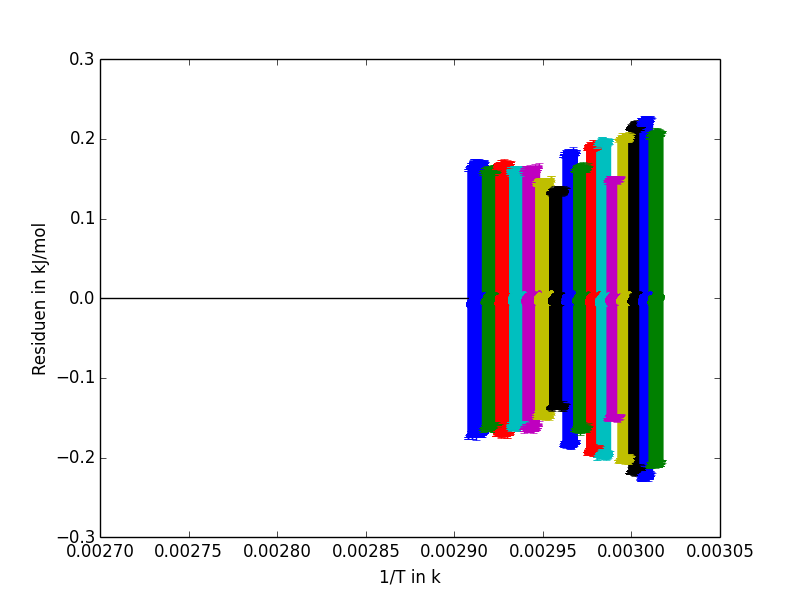
\includegraphics[scale=0.7]{Bilder/residuen_JM_2.png}
\caption{Residuen zur 2. Lineare Regression Hauptmessung Gruppe 1}
\end{figure}
\begin{figure}[H]
\centering
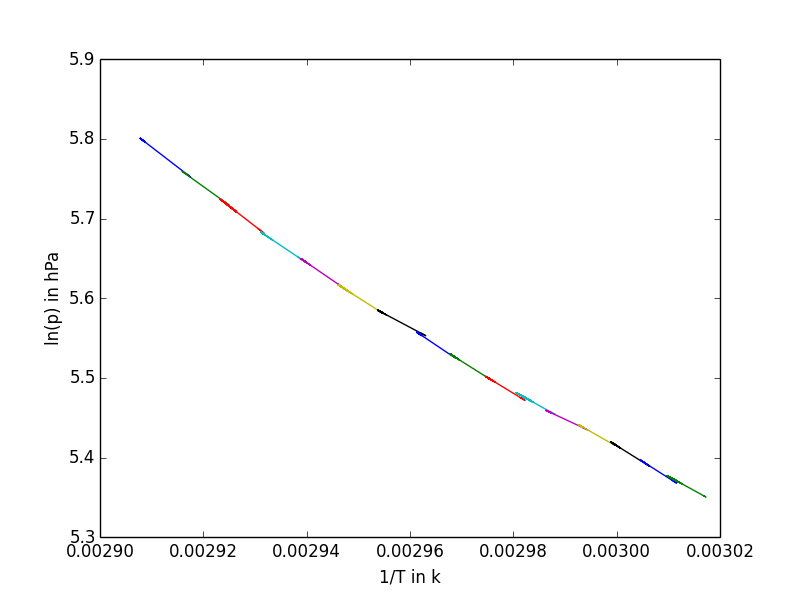
\includegraphics[scale=0.7]{Bilder/linreg_nurlinreg_JM_2.png}
\caption{2. Lineare Regression Hauptmessung Gruppe 1 ohne Messwerte}
\end{figure}
\begin{figure}[H]
\centering
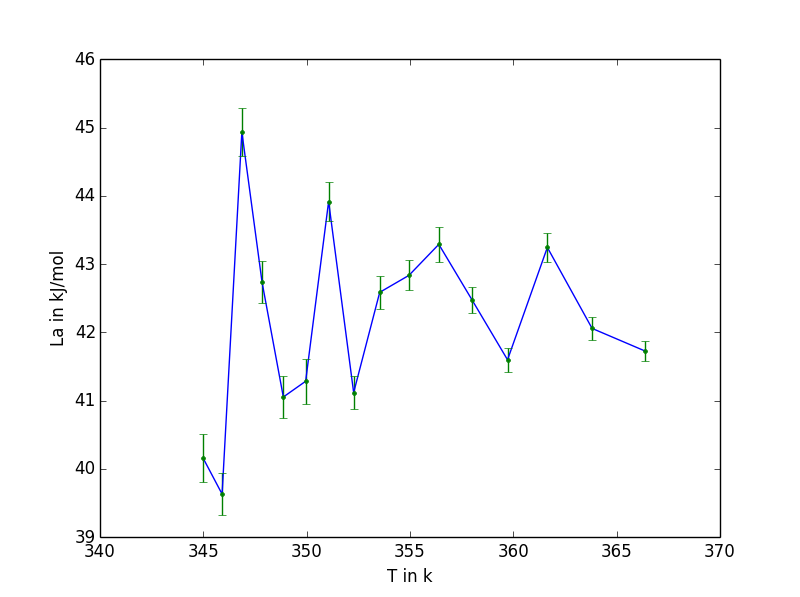
\includegraphics[scale=0.7]{Bilder/lamda_JM_1.png}
\caption{1. $\Lambda$ gegen $T$ Gruppe 1}
\end{figure}
\begin{figure}[H]
\centering
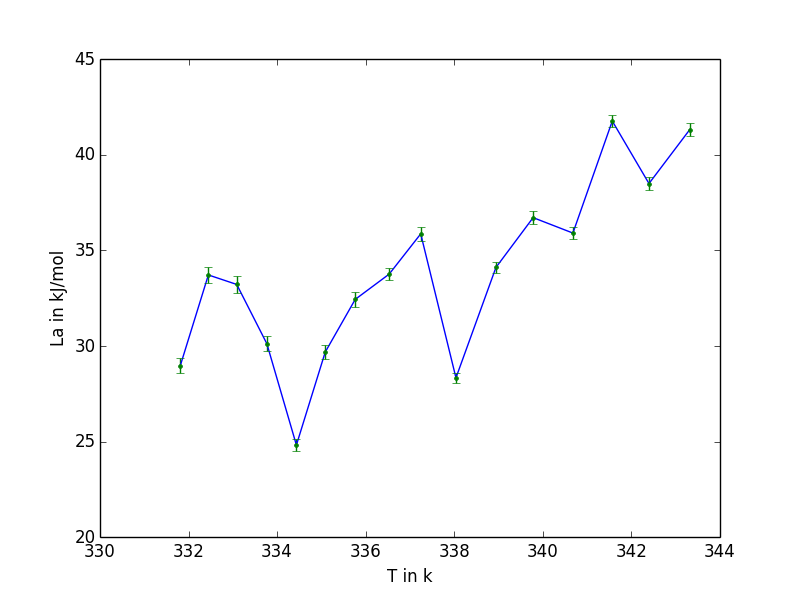
\includegraphics[scale=0.7]{Bilder/lamda_JM_2.png}
\caption{2. $\Lambda$ gegen $T$ Gruppe 1}
\end{figure}

\end{document}